\documentclass[12pt,oneside]{uhthesis}
\usepackage{subfigure}
\usepackage[ruled,lined,linesnumbered,titlenumbered,algochapter,spanish,onelanguage]{algorithm2e}
\usepackage{amsmath}
\usepackage{amssymb}
\usepackage{amsbsy}
\usepackage{caption,booktabs}
\captionsetup{ justification = centering }
%\usepackage{mathpazo}
\usepackage{float}
\setlength{\marginparwidth}{2cm}
\usepackage{todonotes}
\usepackage{listings}
\usepackage{xcolor}
\usepackage{multicol}
\usepackage{graphicx}
\usepackage{multirow}
\usepackage{array}
\newcolumntype{P}[1]{>{\centering\arraybackslash}p{#1}}
\floatstyle{plaintop}
\restylefloat{table}
\addbibresource{Bibliography.bib}
% \setlength{\parskip}{\baselineskip}%
\renewcommand{\tablename}{Tabla}
\renewcommand{\listalgorithmcfname}{Índice de Algoritmos}
%\dontprintsemicolon
\SetAlgoNoEnd

\definecolor{codegreen}{rgb}{0,0.6,0}
\definecolor{codegray}{rgb}{0.5,0.5,0.5}
\definecolor{codepurple}{rgb}{0.58,0,0.82}
\definecolor{backcolour}{rgb}{0.95,0.95,0.92}

\lstdefinestyle{mystyle}{
    backgroundcolor=\color{backcolour},   
    commentstyle=\color{codegreen},
    keywordstyle=\color{purple},
    numberstyle=\tiny\color{codegray},
    stringstyle=\color{codepurple},
    basicstyle=\ttfamily\footnotesize,
    breakatwhitespace=false,         
    breaklines=true,                 
    captionpos=b,                    
    keepspaces=true,                 
    numbers=left,                    
    numbersep=5pt,                  
    showspaces=false,                
    showstringspaces=false,
    showtabs=false,                  
    tabsize=4
}

\lstset{style=mystyle}

\title{Sistema para la Predicción de los \\\vspace{0.25cm} Pronósticos del Mundial de Atletismo}
\author{\\\vspace{0.25cm}Karla Olivera Hernández}
\advisor{\\\vspace{0.25cm}Dr. Yudivián Almeida Cruz}
\degree{Licenciado en Ciencia de la Computación}
\faculty{Facultad de Matemática y Computación}
\date{Noviembre de 2022}
\logo{Graphics/uhlogo}
\makenomenclature

\renewcommand{\vec}[1]{\boldsymbol{#1}}
\newcommand{\diff}[1]{\ensuremath{\mathrm{d}#1}}
\newcommand{\me}[1]{\mathrm{e}^{#1}}
\newcommand{\pf}{\mathfrak{p}}
\newcommand{\qf}{\mathfrak{q}}
%\newcommand{\kf}{\mathfrak{k}}
\newcommand{\kt}{\mathtt{k}}
\newcommand{\mf}{\mathfrak{m}}
\newcommand{\hf}{\mathfrak{h}}
\newcommand{\fac}{\mathrm{fac}}
\newcommand{\maxx}[1]{\max\left\{ #1 \right\} }
\newcommand{\minn}[1]{\min\left\{ #1 \right\} }
\newcommand{\lldpcf}{1.25}
\newcommand{\nnorm}[1]{\left\lvert #1 \right\rvert }
\renewcommand{\lstlistingname}{Ejemplo de código}
\renewcommand{\lstlistlistingname}{Ejemplos de código}

\definecolor{codegreen}{rgb}{0,0.6,0}
\definecolor{alizarin}{rgb}{0.82, 0.1, 0.26}

\begin{document}

\frontmatter
\maketitle

\begin{dedication}

    A mi familia

\end{dedication}
\begin{acknowledgements}
    
    A mis padres, por su paciencia y apoyo incondicional.

    A mis abuelos, por enseñarme a dar siempre lo mejor de mí.
    
    A Ale, por siempre estar ahí.
    
    A Amanda, por acompañarme durante estos años y hacer más livianos los momentos de sufrimiento.
    
    A mis compañeros Victor, Gabi, Luiso, Claudia y todos los que luchamos juntos por estar aquí hoy.
    
    A mis profesores, por ser fuente de inspiración y enseñarnos desde el día uno a amar la carrera. En especial a mi tutor Yudivián, por el apoyo y dedicación brindado hasta el último momento.

\end{acknowledgements}
\begin{opinion}
    
    La estudiante Karla Olivera Hernández desarrolló satisfactoriamente el trabajo de diploma titulado “Sistema para la Predicción de los Pronósticos del Mundial de Atletismo”. En este trabajo la estudiante propuso una metodología para predecir, en base a marcas previas de los atletas, los resultados de los eventos que conformen una determinada competencia de atletismo.

    La propuesta que desarrolló la estudiante se basa en la realización de simulaciones de la competencia donde las marcas que pueda realizar cada atleta se modelan con funciones de distribución de probabilidad, en particular utiliza la Estimación de Densidad de Kernel. Este modelo que propone utiliza un conjunto de parámetros y los resultados que se obtienen están en función de ello. Por eso, para su propuesta, también realiza un proceso de optimización de parámetros contra dos propuestas de funciones a optimizar. Para verificar la viabilidad de su propuesta realiza un conjunto de experimentos. Toma los resultados del mundial de Doha para obtener los parámetros óptimos según el proceso de optimización de parámetros y con esto obtiene las predicciones tanto para los Juegos Olímpicos de Tokio como para el Mundial de Oregón. Estos resultados, a su vez, son comparados con dos modelos parametrizados manualmente que fueron confeccionados previamente para estas dos competencias.
    
    Para poder afrontar el trabajo, la estudiante tuvo que revisar literatura científica relacionada con la temática así como soluciones existentes y bibliotecas de software que pueden ser apropiadas para su utilización. Todo ello con sentido crítico, determinando las mejores aproximaciones y también las dificultades que presentan.
    
    Todo el trabajo fue realizado por el estudiante con una elevada constancia, capacidad de trabajo y habilidades, tanto de gestión, como de desarrollo y de investigación.
    
    Por estas razones pedimos que le sea otorgada a la estudiante Karla Olivera Hernández la máxima calificación y, de esta manera, pueda obtener el título de Licenciado en Ciencia de la Computación.
    \BlankLine
    \BlankLine
    Dr. Yudivián Almeida Cruz

\end{opinion}
\begin{resumen}

	El seguimiento del progreso y las tendencias en algunos deportes permite predecir la dirección en la que se dirige cada disciplina. El presente trabajo se centra en el atletismo y estudia diferentes técnicas para la predicción de los resultados de las modalidades que conforman una determinada competencia. Esto constituye una información muy valiosa tanto para los entrenadores como para los mismos atletas, que buscan lograr actuaciones de alto nivel en los principales eventos internacionales. Particularmente, conocer la posición más probable que ocuparán los atletas en el ranking final puede proporcionar una idea de cuanto se debe reforzar el entrenamiento. Definir una técnica o modelo para realizar estos pronósticos con un rendimiento eficiente y con resultados cercanos a la realidad es una actividad desafiante y compleja, debido a que ninguno es preciso en todos los escenarios. Este trabajo trata de abordar el tema desde una perspectiva diferente. Se presenta una metodología que consiste en la realización de simulaciones de la competencia, donde se hace uso de funciones de distribución de probabilidad para modelar las marcas que pueden obtener los atletas. Este modelo depende de un conjunto de parámetros que influyen directamente en la calidad de los resultados. Es por esto que se propone una técnica de optimización de estos parámetros. Por último, se detallan los aspectos de implementación del prototipo y se evalúan los resultados contra el Campeonato Mundial de Atletismo celebrado en Oregón en el 2022.
	
\end{resumen}

\begin{abstract}

	Tracking progress and trends in some sports makes it possible to predict the direction in which each discipline is headed. This paper focuses on athletics and studies different techniques for predicting the results of the modalities that make up a certain competition. This constitutes very valuable information for both coaches and the athletes themselves, who seek to achieve high-level performances in major international events. In particular, knowing the most likely position that athletes will occupy in the final ranking can provide an idea of how much training should be reinforced. Defining a technique or model to perform these forecasts with efficient performance and with results close to reality is a challenging and complex activity, since none is accurate in all scenarios. This paper tries to address the issue from a different perspective. A methodology is presented that consists in carrying out simulations of the competition, where probability distribution functions are used to model the marks that athletes can obtain. This model depends on a set of parameters that directly influence the quality of the results. For this reason, an optimization technique for these parameters is proposed. Finally, the implementation aspects of the prototype are detailed and the results are evaluated against the World Athletics Championships held in Oregon in 2022.

\end{abstract}
\tableofcontents
% \listoffigures
\listoftables
% \listofalgorithms
\lstlistoflistings

\mainmatter

\chapter*{Introducción}\label{chapter:introduction}
\addcontentsline{toc}{chapter}{Introducción}

El pronóstico de eventos futuros es uno de los trabajos más complicados y desafiantes con los que se ha enfrentado el ser humano a lo largo de su historia. La predicción es una tarea compleja en cualquiera de las áreas del conocimiento en que se aplica y son numerosos los estudios que se han llevado a cabo. Algunos de estos se han dedicado a la predicción de eventos meteorológicos \cite{watson2022improved}\cite{powers2007numerical}, de los futuros cambios en el estado financiero de un país o de una empresa \cite{morris2010measuring}\cite{gilardoni2017recurrent}, de los resultados que se obtendrán en eventos deportivos \cite{vaz2012forecasting}\cite{constantinou2012pi}, del aumento o decremento del valor de las tan revolucionarias criptomonedas \cite{bohte2019comparing}, entre muchos otros más. 

Los sistemas de predicción constituyen uno de los más complejos dentro del campo del análisis de datos. El conocimiento aportado por una buena predicción siempre aporta una ventaja a aquel que sabe hacer uso de él, lo que da mucho valor a las herramientas que pueden predecir con un gran grado de certeza y seguridad qué va a ocurrir en el futuro. Sin embargo, definir una técnica o modelo para realizar estos pronósticos con un rendimiento eficiente y con resultados cercanos a la realidad en diferentes ambientes es una actividad desafiante y compleja, debido a que ninguno es preciso en todos los escenarios.

La práctica de deportes es una parte fundamental en la vida de la mayoría de las personas, lo que hace que el mundo de las estadísticas deportivas esté tan en auge. Para los amantes de un determinado deporte puede resultar muy curioso observar estadísticas acerca de su atleta y equipo favorito o de una competencia en especial. Lo mismo sucede para las personas que realizan apuestas deportivas, conocer los resultados más probables antes de que se lleven a cabo los correspondientes eventos competitivos les puede proveer de un gran beneficio económico. 

Por otra parte, la predicción del rendimiento deportivo puede ayudar a las escuelas, los equipos y las instituciones de deporte a desarrollar métodos de entrenamiento científicos que reflejen las tendencias cambiantes en el rendimiento de los deportistas. Por lo tanto, los atletas y entrenadores podrán utilizar estos resultados como base para reformar la educación y el entrenamiento físico. 

Evaluaciones y análisis de campeonatos mundiales, Juegos Olímpicos y competencias regionales han delineado la dirección que ha asumido el deporte de nuestros días. De manera particular, el atletismo ha sido el foco de varias investigaciones científicas \cite{grubb1998models}\cite{westera2011phenomenology}\cite{godsey2012brian} con el objetivo de desarrollar modelos computacionales que sean capaces de describir el efecto de varios factores que puedan influir en el rendimiento e incluso puedan predecir futuros resultados.

Algunos científicos proyectan la evolución de las distintas marcas en función de las estadísticas de los últimos 100 años y establecen un patrón que tiene en cuenta factores fisiológicos y límites biomecánicos \cite{kumarforecasting}\cite{mishra2013mathematical}. Pero, cuando entra en juego el comportamiento humano como factor fundamental, a veces los datos no son suficientes para predecir con garantías la capacidad del ser humano para superarse. Ejemplo de esto es lo ocurrido en el año 2008 cuando el jamaicano Usain Bolt, además de pulverizar tres récords del mundo en unas Olimpiadas, puso de patas arriba todos los modelos matemáticos de predicción elaborados hasta esa fecha. En uno de los gráficos con las predicciones de la prueba de 100 metros lisos hasta el año 2100, se describía una curva de evolución descendente que venía cumpliéndose de forma escrupulosa hasta el momento. El atleta jamaicano se adelantó a la predicción en 20 años y alcanzó la marca de 9.69 segundos que los matemáticos habían previsto para el año 2030 \cite{wired}.

\subsection*{Motivación}

Existen diferentes plataformas que se dedican a investigar y pronosticar los posibles resultados de cada país en importantes eventos como los Juegos Olímpicos y los Campeonatos Mundiales de Atletismo. Algunas de estas plataformas son Gracenote Sports Virtual Medal Table \cite{gracenote}, que utiliza un algoritmo para clasificar a los atletas y equipos en cada evento olímpico en función de los resultados de competencias recientes, y BEST Sports \cite{bestsports}, que publica predicciones de resultados deportivos generados por expertos que utilizan modelos estadísticos y algoritmos de aprendizaje automático. Ambas plataformas solo hacen predicciones de la tabla final de medallas, sin llegar a presentar un podio con los atletas que tengan mayor probabilidad de ocupar las primeras posiciones.  

Por otro lado, muchas han sido las investigaciones encaminadas a la predicción de futuros resultados obtenidos por atletas, pero solo se enfocan en el estudio de algunas disciplinas en específico y no proponen un modelo que logre abarcar todas las modalidades del atletismo \cite{girardi2022performance}. Además, muchos de esos estudios no solo trabajan con las marcas personales de los atletas, sino que también con otras métricas como velocidades máximas alcanzadas en el caso de las carreras de velocidad y variables relacionadas con el metabolismo y con las características fisiológicas de los deportistas \cite{zhou2022sports}\cite{mulligan2018minimal}.

Un sistema de predicción de las diferentes modalidades del atletismo ayudaría en la selección de la delegación deportiva que representará a cada país con el fin de lograr las mejores posiciones en los podios. Además, se lograrían constantes mejoras de los deportistas a través de la adaptación de nuevos hábitos de entrenamiento o incrementando el rendimiento de los equipos al utilizar estrategias más complejas, realistas y personalizadas.  A la vez, permitiría comprender los límites reales de la capacidad humana para establecer objetivos nuevos y sensatos que los atletas deberán alcanzar, para así proporcionar una comprensión más coherente de lo que sugieren las actuaciones del pasado sobre las actuaciones del futuro.

\subsection*{Antecedentes}

En el grupo de investigación de Inteligencia Artificial de la Facultad de Matemática y Computación de la Universidad de la Habana se han realizado trabajos para obtener pronósticos de diferentes deportes dentro de los Juegos Olímpicos celebrados en Tokio 2020 \cite{tokio2020}. En el caso de la predicción de las distintas modalidades del atletismo, los resultados obtenidos no fueron muy certeros. De las 43 disciplinas pronosticadas, hubo 70 medallistas pronosticados correctamente de 129 y, de ellos, 23 posiciones exactas.  

\subsection*{Problemática} 

Los modelos de predicción del atletismo existentes en la actualidad solo se enfocan en una cuestión en específico, sin llegar a ser del todo abarcadores. Algunos solo hacen predicciones de la tabla final de medallas en las competencias, mientras que otros se enfocan en predecir las futuras marcas que obtendrán los atletas en un determinado certamen. Ninguna de estas dos vías logra, dentro de una competencia, construir un ranking final para cada disciplina con los atletas que tengan la mayor probabilidad de ocupar las primeras posiciones.

En vistas a la materialización de esta investigación, se propone como hipótesis que la implementación de un sistema de predicción basado en simulaciones y contando solo para cada atleta con resultados obtenidos en ediciones de competencias anteriores, es capaz de obtener pronósticos, lo más cercanos posible, de los resultados de las diferentes competiciones de atletismo.

El mecanismo principal que se presenta para la predicción es la realización de una serie de simulaciones de cada disciplina, donde se crea una función para cada atleta capaz de aprender de registros históricos para la generación de nuevos resultados que son altamente probable que se obtengan. Por último, se realiza un estudio estadístico para brindar una propuesta de ranking final.

La simulación permite cambiar casi cualquier entrada al proceso de pronóstico y, casi en tiempo real, ver qué impacto tendría en los resultados; y en caso de que se presente alguna mejora, modificar según sea necesario. Los resultados obtenidos serán comparados con el Campeonato Mundial de Atletismo 2022 celebrado en Oregón con el objetivo de evaluar el rendimiento y precisión del sistema.

\subsection*{Objetivos}

El \textbf{objetivo general} consiste en proponer una metodología que permita predecir la posición que ocuparán los atletas en el ranking de cada una de las modalidades que conformen una competencia de atletismo.

Para alcanzar el cumplimiento del objetivo general se plantean una serie de \textbf{objetivos específicos}:

\begin{enumerate}
\item Estudiar diferentes modelos de predicción para algunos eventos deportivos presentes en la literatura, en especial los del atletismo, así como sus enfoques para resolver la problemática presentada.
\item Proponer un método que permita modelar la función de resultados de cada atleta, que aprenda de marcas obtenidas en competencias anteriores y sea capaz de generar nuevas.
\item Diseñar e implementar un prototipo de sistema de predicción que construya el ranking más probable para cada modalidad del atletismo.
\item Evaluar experimentalmente la eficacia de la metodología propuesta, tomando en cuenta los resultados obtenidos por el sistema implementado.
\end{enumerate}

\subsection*{Organización de la tesis}

El resto del documento se encuentra estructurado en tres capítulos que proporcionan una explicación detallada de las diferentes fases por las que transitó el desarrollo del presente trabajo. En el capítulo \ref{chapter:state-of-the-art} ``Estado del Arte'' se realiza un estudio de las diferentes investigaciones realizadas y modelos propuestos hasta la fecha que más se acercan a la problemática presentada. En el capítulo \ref{chapter:proposal} ``Propuesta'' se describe de forma general la concepción y el diseño de la solución y se explica detalladamente la metodología propuesta para obtener las predicciones. En el capítulo \ref{chapter:implementation} ``Detalles de Implementación y Experimentos'' se detallan los aspectos técnicos seguidos en la implementación del prototipo, así como las herramientas utilizadas, y se hace un análisis de los resultados obtenidos en el proceso de experimentación. Para finalizar, se exponen las conclusiones de la investigación, seguido de algunas recomendaciones para investigaciones y trabajos futuros. Al final del documento se presentan algunos anexos y todas las referencias bibliográficas de los trabajos consultados.
\chapter{Estado del Arte}\label{chapter:state-of-the-art}

La Ciencia de Datos es uno de los términos que más está presente cada vez que se habla sobre las nuevas tecnologías y las herramientas de análisis más usadas en la actualidad. Hayashi en 1998 \cite{hayashi1998} define el concepto de Ciencia de Datos como el campo de estudio que pretende analizar y comprender los fenómenos reales con datos. En otras palabras, su objetivo es revelar las características o la estructura oculta de aquellos fenómenos naturales, humanos y sociales complicados a través de los datos, desde un punto de vista diferente de la teoría y métodos tradicionales. 

En esencia, la Ciencia de Datos combina múltiples campos para lograr el cumplimiento de su más crucial objetivo, que es la extracción de conocimiento de los datos, entre los que se incluyen métodos científicos, estadísticos, análisis de datos y modelos de inteligencia artificial. Sus aplicaciones más comunes son el modelado predictivo, el reconocimiento de patrones, la detección de anomalías, la clasificación, la categorización y el análisis de sentimientos; así como el desarrollo de tecnologías como motores de recomendación, sistemas de personalización y herramientas de inteligencia artificial.

Dentro del sector deportivo, el análisis de datos se ha convertido en una herramienta poderosa. La accesibilidad de los datos en forma de resultados generados en los distintos eventos deportivos en un año específico permite el análisis de actuaciones en cualquier competencia. A partir de los análisis de estos resultados se pueden observar cambios en el rendimiento de los deportistas a lo largo del tiempo y se pueden hacer predicciones de rendimiento futuro utilizando modelos matemáticos y computacionales.  

Entre sus múltiples aplicaciones en el sector del deporte se destacan la predicción de la tabla de medallas en importantes competencias, la predicción de los resultados de varios eventos por equipos y de eventos individuales en modalidades como el atletismo.

\section{Predicción de tabla de medallas}

Varios autores han dedicado parte de su trabajo a estudiar y pronosticar los posibles resultados de cada país en importantes eventos, como pueden ser los Juegos Olímpicos, los Campeonatos Mundiales de Atletismo, entre otros.

Unos de los primeros investigadores en abordar este tema fueron Kuper y Sterken en el año 2001, que proporcionaron una metodología para la obtención de los pronósticos de medallas y la participación en los Juegos Olímpicos tanto de Invierno \cite{kuper2001olympic} como de Verano \cite{kuperolympicgerard}, presentando resultados separados para eventos antes y después de la Segunda Guerra Mundial. Su enfoque principal es el impacto de los determinantes económicos, geográficos y demográficos de la participación y el éxito olímpico. Su método consiste en estimar primero la participación y luego modelar el rendimiento olímpico en términos de reparto de medallas de oro, plata y bronce, este último, condicionado a la participación. Además, agregaron nuevas variables para representar si es o no el país anfitrión, el ingreso per cápita y la clasificación de algunos países según sus sistemas legales.

Asimismo, Johnson y Ali en el 2004 \cite{johnson2004tale} en su búsqueda por determinar las influencias estructurales de la participación y el éxito de un país en los Juegos Olímpicos, llegaron a la existencia de una ventaja significativa y medible para las naciones más grandes y de mayores ingresos. Entre las naciones participantes, las naciones de altos ingresos siempre se desempeñan muy bien en el recuento de medallas, aunque los efectos son más pronunciados en el verano debido a la diferencia en la cantidad de participantes. Curiosamente, las naciones pequeñas superan a sus competidores más grandes en los Juegos de Invierno, mientras que lo contrario es definitivamente cierto en los Juegos de Verano. 

Como se demostró en los artículos anteriores, las características demográficas y económicas brindan un poder predictivo importante para determinar el éxito de un país en los Juegos Olímpicos. Bernard y Busse en el 2004 \cite{bernard2004wins} y Pfau en el 2006 \cite{pfau2006predicting}, ampliaron dicha investigación haciendo uso de métodos de la economía y la econometría, con el fin de demostrar el poder de un modelo econométrico simple. Bernard y Busse hacen uso de una función de producción Cobb-Douglas para representar a la población y al ingreso nacional en la producción de talento olímpico (la cantidad de atletas que se presentan en la competencia) por país, y de una función logarítmica para la traducción de este talento relativo en la cantidad de medallas ganadas. Pfau se basó en el estudio anterior y lo extendió añadiendo variables propuestas por otros autores mencionados anteriormente, llegando a construir un modelo más completo.

Schlembach y col. en el 2020 \cite{schlembach2020forecasting} atacaron dicho problema desde una perspectiva más moderna haciendo uso de aprendizaje automático para aumentar significativamente la precisión del pronóstico de medallas olímpicas. Su modelo consiste en un Random Forest de dos etapas que según, los experimentos realizados por los autores, supera por primera vez el método de pronóstico naïve más tradicional para tres Juegos Olímpicos celebrados entre 2008 y 2016. Este estudio no es el único en aplicar este enfoque, Jia y col. también utilizan modelos de regresión para ajustar la lista de medallas: el modelo GBR, el modelo de regresión polinomial y Random Forest. Coinciden también, luego de haber entrenado y evaluado los tres modelos, en que Random Forest es el que mejor se ajusta y obtiene las predicciones más cercanas a la realidad.

El seguimiento del progreso y las tendencias en algunos deportes permite predecir la dirección en la que se dirige cada disciplina. Hay investigaciones que no solo se han dedicado al pronóstico de las tablas de medallas, sino que han tratado de ir un poco más allá y modelar a equipos o deportistas en específico para predecir futuros resultados que puedan obtener en enfrentamientos o competencias. De esta forma no solo se puede conocer la cantidad de medallas que obtiene un país, sino además el lugar más probable que ocupe cada uno de sus deportistas en el podio final. La mayoría de estos trabajos se han bifurcado en dos vertientes, los que se centran en el estudio de los parámetros que más valor atribuyen a la modelación de los equipos y los que se centran en los parámetros de los deportistas individuales. 

\section{Predicción de eventos por equipos}

En el fútbol, Piza \cite{piza2005futbol} presenta una metodología para la estimación de las probabilidades de clasificación de una selección en importantes competencias como el Mundial de Fútbol. Se trata de un modelo matemático del tipo simulación de Monte-Carlo, a través del cual se realizan millones de simulaciones de los posibles resultados de los juegos pendientes en un torneo de fútbol (siguiendo ciertas leyes de probabilidad), en el cual solamente un número limitado de equipos puede obtener la clasificación a la siguiente etapa de la competencia. El modelo toma en consideración los principales factores que pueden influir en los resultados en este contexto, tales como por ejemplo la historia reciente, el potencial actual de los equipos y las circunstancias particulares que rodean los partidos pendientes.

Vázquez y col. \cite{vazquez2014combining} generan un modelo de predicción de resultados de partidos de baseball mediante la comparación de estadísticas a lo largo del tiempo. Los autores toman en consideración que los equipos que actúan de manera similar se desempeñarán de manera similar en situaciones concretas con una alta probabilidad. De la misma manera, asumen que los juegos deben desarrollarse de manera similar si los equipos que juegan son similares. La propuesta que presentan combina series temporales y algoritmos de agrupamiento para generar un modelo que aprende de la evolución de equipos y partidos e intenta predecir resultados finales.

Thabtah y col. \cite{thabtah2019nba} proponen un marco de aprendizaje automático para predecir los resultados de los juegos en la NBA con el objetivo de descubrir el conjunto de características influyentes que afectan estos resultados. Para identificar si los métodos de aprendizaje automático son aplicables en el pronóstico del resultado de un juego de la NBA utilizando datos históricos (juegos anteriores), y cuáles son los factores significativos que afectan el resultado de estos, se seleccionan varios métodos de aprendizaje automático que utilizan diferentes esquemas de aprendizaje para derivar los modelos, incluidos Naïve Bayes, redes neuronales artificiales y Decision Tree. 

\section{Predicción de eventos individuales}

Ho{\l}ub y col. \cite{holub2021predicting} analizan los resultados de los finalistas, ganadores y últimos participantes en las finales de mujeres y hombres de natación y crean un modelo predictivo matemático. Como parte de su trabajo analizaron los resultados obtenidos a lo largo de toda la historia de los Juegos Olímpicos y luego aplicaron en la producción de un modelo matemático predictivo, basado en análisis de regresión lineal univariado, para calcular los tiempos estimados de los ganadores, finalistas y últimos participantes en las finales olímpicas de Tokio 2021.

Kholkine y col. \cite{kholkine2021learn} utilizan datos fácilmente accesibles sobre ciclismo de ruta de los últimos 20 años y la técnica de aprendizaje automático Learn-to-Rank (LtR) para predecir los 10 principales contendientes para carreras de ciclismo de ruta de 1 día. Esto lo lograron asignando un peso de relevancia al lugar final en las primeras 10 posiciones y evaluando el rendimiento de este enfoque en las ediciones de 2018, 2019 y 2021 de seis carreras clásicas de primavera de 1 día. Al final compararon el resultado con una predicción masiva de fanáticos. Las métricas que utilizaron fueron la ganancia acumulativa descontada normalizada (NDCG) y la cantidad de 10 conjeturas principales correctas. Finalmente, descubrieron que su modelo, en promedio, tiene un rendimiento ligeramente superior en ambas métricas que la predicción de fanáticos masivos. También analizaron qué variables de su modelo tienen más influencia en la predicción de cada carrera.

Por otra parte, Liu y col. \cite{liu2022construction} estudiaron el evento de patinaje de velocidad completo femenino, un sistema de competencia complejo y desafiante para hacer predicciones precisas sobre su desempeño. Usaron seis algoritmos de ML diferentes: Support Vector Machine (SVM), Logistic Regression (LR), Random Forest (RF), K-Nearest Neighbor (KNN), Naive Bayes (NB) y Neural Network (NN) para construir un Modelo de Carrera de 5.000 m. Luego, el rendimiento y la funcionalidad de estos modelos se examinaron y compararon explícitamente. El resultado del modelo concluía si el atleta podía participar en la competencia de 5000 o ganar una medalla. En la evaluación y comparación del modelo de carrera y del modelo de medalla, SVM obtuvo la clasificación más equilibrada a través de una comparación exhaustiva de precisión.

\section{Predicción de eventos del atletismo}

Durante la preparación y entrenamiento de los atletas en deportes como el atletismo, es frecuente que los entrenadores se interesen por predecir su rendimiento. Con este fin, numerosos científicos han desarrollado modelos matemáticos, estadísticos y de inteligencia artificial que logran describir el efecto de varios factores en el rendimiento de los atletas, logrando predecir incluso resultados futuros. 

\subsection{Modelos matemáticos y estadísticos}

La modelación matemática es definida por Anhalt y col. \cite{anhalt2018mathematical} como el proceso de seleccionar y utilizar las matemáticas a través de una simplificación de la realidad que se expresa en un lenguaje simbólico tomando la forma de ecuaciones, algoritmos y relaciones gráficas. Algunos han utilizado modelos lineales para trazar y predecir el cambio del rendimiento de los atletas, mientras que otros han utilizado métodos de estimación de curvas múltiples basados en funciones inversas, sigmoides, cuadráticas, cúbicas, compuestas, logísticas, de crecimiento y exponenciales.

Las investigaciones de Hill en 1925 \cite{hill1925physiological} y Keller en 1973 \cite{keller1973theory} se centraron en los corredores de distancia y desarrollaron modelos basados en el metabolismo para proporcionar una explicación fisiológica de la relación tiempo-distancia y predecir el rendimiento récord. En el caso de Hill se trata de responder a la interrogante “¿Qué tan rápido puede correr un atleta una cierta distancia?”, teniendo en cuenta el factor fatiga. Mientras que, por otro lado, Keller ajusta la curva teórica a cuatro registros observados: la fuerza máxima que puede ejercer un corredor, la fuerza resistiva que se opone al corredor, la velocidad a la que el metabolismo del oxígeno suministra energía y la cantidad inicial de energía almacenada en el cuerpo del corredor al comienzo de la carrera. 

Grubb en 1998 \cite{grubb1998models} para determinar las fortalezas de un atleta y evaluar el efecto del entrenamiento, propuso una forma paramétrica que caracteriza el cambio del rendimiento de los corredores con la distancia. La definición que planteó como rendimiento fue la velocidad promedio para cada distancia, lo cual permite hacer análisis que ayuden a predecir rendimientos futuros.

Heazlewood en 2006 \cite{heazlewood2006prediction} hizo uso de ecuaciones matemáticas que dependen de los tiempos obtenidos y las distancias reales logrados por los atletas para la predicción de los eventos de 100 m, 400 m, salto de longitud y salto de altura masculino y femenino. Para investigar las hipótesis de ajuste y predicción del modelo, once modelos de regresión se aplicaron individualmente a cada uno de los eventos atléticos y de natación. Por último, la ecuación de regresión que produjo el mejor ajuste para cada evento fue la escogida, para lo cual se apoyaron en el cálculo del coeficiente de determinación (R2). Tanto para los 100 m masculinos como para el salto largo femenino escogieron una función inversa, para los 100 m femeninos y el salto largo masculino una función cúbica, una función sigmoide para los 400 m tanto masculinos como femeninos y para el caso del salto alto, dieron iguales resultados la función exponencial, de crecimiento, compuesta y logística.  

En el 2008, Joyner y Coyle \cite{joyner2008endurance} realizan una revisión de los factores que interactúan en los deportes de resistencia y su utilidad como predictores del rendimiento de elite. Los factores que marcan como principales son: el consumo máximo de oxígeno (VO2, máx.), el llamado "umbral de lactato" y la eficiencia (el costo de oxígeno para generar una velocidad de carrera dada o una producción de potencia de ciclismo); que parecen desempeñar un papel clave en el rendimiento de resistencia.

Westera \cite{westera2011phenomenology} presentó un Modelo Predictor Personal para las carreras de velocidad, el cual solo utiliza dos marcas personales de un atleta para la calibración y permite luego predecir las marcas personales hipotéticas de un atleta para cualquier otra distancia.

Galván y col \cite{galvanmathematical} propusieron diferentes modelos matemáticos para algunos eventos del atletismo. Se crearon cinco ecuaciones a partir de los datos reales: una ecuación polinómica de quinto orden para el maratón masculino, una ecuación polinomial de quinto orden para el maratón femenino, una ecuación polinomial de segundo orden para la marcha masculina de 20 km, una ecuación de potencia para la marcha de 20 km de mujeres, y una ecuación polinomial de segundo orden para la marcha de 50 km de hombres.

\subsection{Modelos basados en datos}

La relación entre un modelo matemático y la realidad tiene fuertes implicaciones en cuanto a la percepción del mundo y las interpretaciones de los resultados por los científicos, por lo que pronosticar el éxito depende de seleccionar un método apropiado y altamente preciso. Es por esto que varios autores han incursionado en otras vías de estudio para la predicción: los modelos basados en datos. Con los modelos basados en datos no es necesario determinar de antemano la expresión matemática que va a representar el modelo de predicción de rendimiento único de un atleta; sino, por el contrario, se trata de hacer uso de herramientas que aprendan por si solas la mejor vía para representar los datos.

Godsey \cite{godsey2012brian} no se enfocó en la predicción de las marcas futuras de un atleta en específico, sino en predecir la calificación máxima esperada en un evento determinado y tanto la probabilidad de que se supere una marca específica como el número esperado de dichas actuaciones en un período de tiempo determinado. Propusieron un algoritmo sencillo y basado en modelos para asignar puntuaciones a actuaciones deportivas, las cuales se basan en el número esperado de atletas que se desempeñan mejor que una marca dada dentro de un año calendario. Para esto, de forma general, estiman una distribución logarítmica normal para cada evento deportivo $k$ usando una lista de las mejores $n_k$ marcas de ese evento y asumen que los logaritmos naturales de los rendimientos de cada evento se distribuyen normalmente.

Las herramientas de Inteligencia Artificial también han proporcionado muy buenos resultados a la hora de predecir rendimientos futuros. Blythe y Király en el año 2016 \cite{blythe2016prediction} trataron de proponer un modelo que explicara simultáneamente la fisiología individual y el rendimiento colectivo de los corredores. Su enfoque basa las predicciones en Local Matrix Completion (LMC), una técnica de aprendizaje automático que postula la existencia de un pequeño número de variables explicativas que describen el rendimiento de los corredores individuales. En su estudio, descubrieron que un resumen de tres números para cada individuo explica el rendimiento en toda la gama de distancias, desde los 100 m hasta el maratón. El resumen de tres números se relaciona con: la resistencia de un corredor, el equilibrio relativo entre velocidad y resistencia, y la especialización en distancias medias.

Zhou en el 2022 \cite{zhou2022sports} propuso un método para predecir con precisión el rendimiento deportivo basado en Redes Neuronales Profundas, el cual se basa en una relación funcional entre el rendimiento deportivo de los atletas y sus indicadores de entrenamiento: índices de forma corporal, función, calidad básica y calidad especial.

Son numerosos los trabajos enfocados en la predicción de los resultados que obtendrán los atletas en disímiles y futuros eventos deportivos. Algunos proponen modelos sencillos para alguna modalidad en específico del atletismo, estudiando solamente marcas de los deportistas y buscando funciones matemáticas que mejor puedan describir el comportamiento que siguen. Existen otros que llevan a cabo un estudio exhaustivo, trabajando con variables relacionadas con la psicología y fisiología de los atletas, con el objetivo de llegar a obtener predicciones más exactas. Otros, necesitan de la intervención de expertos para poder ajustar estos modelos, sin llegar a aprovechar la información que puede suministrar los resultados finales de competencias pasadas.

Aun cuando el abanico de técnicas que se han aplicado es muy amplio, no ha disminuido el interés de los investigadores en seguir proponiendo nuevos enfoques para solucionar este problema. La presente investigación es uno de ellos y se propone como objetivo principal presentar una nueva metodología para la construcción de un sistema de predicción de las diferentes modalidades del atletismo. Se quiere verificar que tan bueno puede ser un modelo que cuente solo con marcas obtenidas por los atletas en el pasado y sea capaz de ajustar sus valores a partir de resultados de competencias ya celebradas. Se propone un nuevo enfoque con respecto a los estudiados anteriormente, que será explicado detalladamente en los próximos capítulos.
\chapter{Propuesta}\label{chapter:proposal}

En el presente capítulo se presenta la metodología empleada para la predicción de los resultados de las diferentes eventos del atletismo en importantes competencias. Se expone el estudio realizado sobre el conjunto de datos necesarios, la modelación de las marcas de los atletas, la idea detrás del algoritmo de predicción y, por último, el proceso de optimización para escoger el valor de algunos parámetros importantes que influyen en las predicciones finales sin necesidad de contar con criterios de experto. 

\section{Concepción general de la solución}

En este trabajo se propone una metodología que permita predecir la posición que ocuparán los atletas en el ranking final de cada uno de los eventos de una competencia de atletismo. Para esto, se concibe la estructura general del proceso de predicción con las siguientes etapas: captura de los datos de una fuente fiable, preprocesamiento y limpieza de los datos, modelado de una función de los resultados para cada atleta y, por último, la ejecución de simulaciones junto con un estudio estadístico de los resultados para brindar una propuesta final de pronóstico para cada evento. (Figura \ref{fig:diagram1})

\begin{figure}[H]
    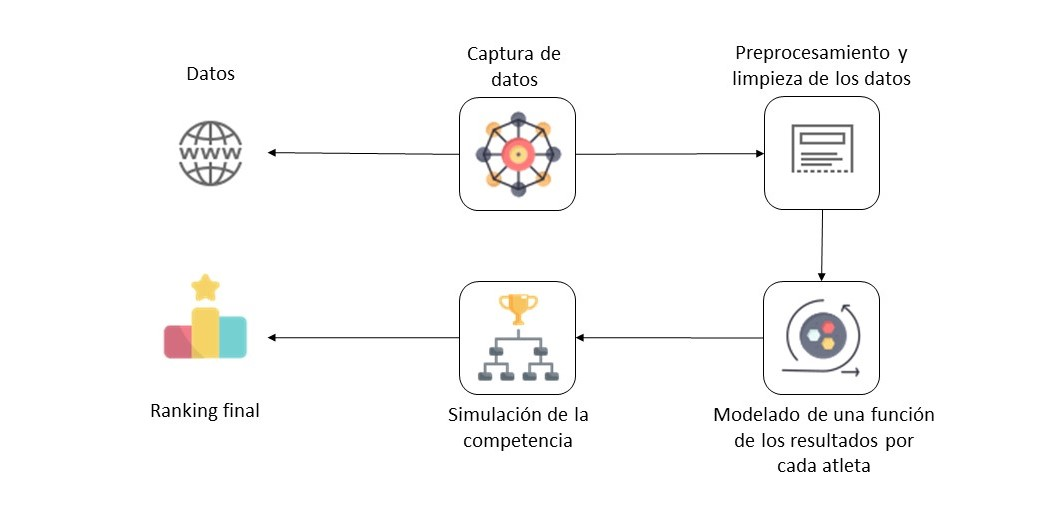
\includegraphics[width=\linewidth]{Graphics/diagram1.jpg}
    \caption{Pipeline de la metodología propuesta para la predicción del ranking final de los diferentes eventos que conforman una competencia de atletismo}
    \label{fig:diagram1}
\end{figure}

\subsection{Captura y preprocesamiento de los datos}

El sistema de predicción que se propone se basa únicamente en resultados obtenidos por los atletas en competencias pasadas para la construcción del ranking más probable de cada evento. Por esta razón, en un primer momento, es primordial definir cuáles son los datos con los que se va a trabajar.

Para una competencia en específico, se requiere conocer los datos expuestos a continuación: 

\begin{itemize}
    \item El nombre de la competencia.
    \item La fecha de inicio de la competencia, importante para la validación de las marcas de los atletas, ya que se desea ser lo más transparente y justo posible en el proceso de predicción y no tomar marcas posteriores al comienzo de la competencia.
    \item Las disciplinas que forman parte de la competencia y sus modalidades (masculino y femenino); es necesario conocerlas todas, puesto que cada una se analizará de manera individual.
    \item Para cada disciplina, si el objetivo de los atletas es obtener la mayor o menor marca, dato importante para la construcción de los rankings.
    \item La lista de nombres de los atletas que se presentarán en cada una de las modalidades.
    \item De cada atleta su nombre, país al que representa y las marcas obtenidas en un número determinado de competencias previas, importante para la construcción de la función de sus resultados.
\end{itemize}

\subsection{Modelado de la función de resultados de un atleta}

Como se ha podido comprobar en la bibliografía consultada en el capítulo anterior, la creación de modelos capaces de obtener posibles resultados futuros de los atletas y consecuentes con sus actitudes pasadas se ha atacado desde varias perspectivas. Muchos se han basado en diferentes datos recopilados, como es el caso de las marcas personales obtenidas, velocidades máximas alcanzadas en el caso de las carreras de velocidad y variables relacionadas con el metabolismo y con las características fisiológicas de los atletas.

El objetivo de esta investigación es poder construir un modelo que solo cuente con las marcas personales de los atletas para la predicción de futuros resultados. Una idea es encontrar una variable aleatoria que pueda describir los resultados de un atleta en un evento en particular y en un tiempo dado. Para que esta variable sea capaz de generar resultados nuevos, es importante encontrar primero una distribución de probabilidad que la caracterice. Una alternativa posible para encontrar esta distribución es modelarla a partir de métodos de estimación de densidad.

Los métodos de estimación de densidad son herramientas estadísticas que se utilizan para reconstruir o estimar una función de densidad de probabilidad (PDF) desconocida a partir de un conjunto de muestras extraídas. Estos estimadores se clasifican en paramétricos y no paramétricos. Un estimador no paramétrico no utiliza suposiciones a priori sobre la distribución subyacente para obtener estimaciones sobre esta distribución. En comparación, un estimador paramétrico asume la forma funcional de la PDF subyacente y utiliza las muestras u observaciones para obtener estimaciones de los parámetros que definen la forma de la PDF. Un ejemplo de un estimador paramétrico sería asumir que la forma de la PDF que se estima es gaussiana y usar las muestras para obtener estimaciones de la media y la desviación estándar de la distribución gaussiana. Los estimadores no paramétricos no hacen suposiciones sobre la forma de la distribución y, por lo tanto, son herramientas más flexibles para capturar distribuciones donde no se conoce información suficiente a priori \cite{burke2016kernel}.

Uno de los estimadores no paramétricos más empleados es la Estimación de la Densidad del Kernel (KDE) \cite{rosenblatt1956remarks}. Dado un valor  $x_i$  la función aprendida por KDE devuelve la densidad de la distribución en el punto  $x_i$ . Esta densidad, cuyo valor está acotado al rango $[0, + \infty )$, es una medida relativa de verosimilitud (likelihood). Si la densidad para el punto A es mayor que la de B, significa que la probabilidad de que A pertenezca a la distribución es mayor que la de B. Esta técnica permite crear una curva suave dado un conjunto de datos aleatorios. La estimación también se puede usar para generar puntos que solo parecen provenir de un conjunto de muestras específico. Esta característica es particularmente útil en el presente trabajo y la razón principal por la que KDE fue escogida.

La definición formal de KDE, dado un conjunto de muestras $ X_1, \cdots, X_n $ de una PDF subyacente, es: 

\begin{equation}
    \label{eq:kde}
    \hat{p_n} (x) = \frac{1}{nh} \sum_{i=1}^{n} K (\frac{X_i - x}{h})
\end{equation}
 
donde $K(x)$ se denomina función kernel, que define la forma y la distribución de la influencia (peso) que se asocian a cada observación y $h > 0$ se denomina ancho de banda, que controla la cantidad de suavizado (cuánto se expande la influencia de cada observación). Básicamente, el KDE suaviza cada punto de datos $X_i$ en pequeñas protuberancias de densidad y, luego, suma todas estas pequeñas protuberancias para obtener la estimación de densidad final.

El ancho de banda $h$ es un parámetro fundamental a la hora de utilizar KDE. Si el ancho de banda es muy pequeño reproduce detalles de los datos que son insignificantes y se adjudican a ruido estadístico debido a que es una cantidad de muestras finita. Por otro lado, si el ancho de banda es muy grande se genera un sobre-suavizado que puede hacer que se pierdan de vista algunas características de la distribución. Por lo tanto, la elección de un ancho de banda se trata de una relación de compromiso entre no reproducir ruido estadístico y una buena descripción de la distribución. 

Luego de definir formalmente a KDE y hacer un análisis de sus características y las ventajas que posee, es seleccionado para la modelación de la función de resultados de cada atleta. La función de kernel escogida para definir la forma y la distribución de la influencia que se asocian a cada observación es la gaussiana. Por otro lado, el análisis de los datos para escoger el mejor valor de ancho de banda a menudo se ha realizado mediante un enfoque de prueba y error. Si se pudiera acordar un método eficiente que, usando los datos, permitiera determinar de forma automática este valor, la utilidad de KDE mejoraría enormemente. La vía propuesta para escoger este valor se explica en la sección \ref{sec:params_opt}.

En aras de poder construir el mejor modelo que represente al atleta en el momento de la competencia, se hace uso solo de marcas obtenidas en una cantidad específica de años anteriores al momento que se desea predecir. Además, se realiza un trabajo de preprocesamiento con el vector de resultados para cada atleta, mediante una ponderación de los años escogidos, donde se les asigna un mayor peso a los años más recientes. De esta forma, si la competencia se lleva a cabo en el año 2022 y se toman $n$ años, solo se escogen las marcas de los años $ 2022,\ 2021, \cdots,\ 2022 - (n-1)$ y a cada año se le asigna un peso $w$. Por tanto, para el entrenamiento del modelo se le pasan las marcas del año 2022 repetidas $w_{2022}$ veces, las del año 2021 aparecerán $w_{2021}$ veces y así en adelante. 

Uno de los problemas que puede aparecer una vez se analizan los datos extraídos es que existe una gran ambigüedad en aquellos casos de atletas con muy pocas marcas registradas. Puede existir el caso de que un atleta tenga una sola marca muy buena registrada, pero solo haberla obtenido en una ocasión, lo cual no se puede considerar muy confiable. Es por esto que se propone agregar, además, un parámetro \textit{alpha} que modifique las marcas de la siguiente manera:

\begin{equation}
    \label{eqn:alpha1}
    pondVal = (1 + \frac{alpha}{cantMarcas}) 
\end{equation}
\begin{equation}
    \label{eqn:alpha2}
    marca_i = marca_i * pondVal
\end{equation}

Esto permite premiar a aquellos atletas que cuentan con un mayor número de marcas, ya que en ese caso es más confiable el hecho de que se repitan. De esta forma, mientras menos marcas tiene un atleta mayor será el valor resultante de cada marca (para eventos donde se busca maximizar el valor de la marca se toma \textit{alpha} negativo).

Una vez ya se tienen definidos los parámetros de KDE y las marcas preprocesadas de los atletas, se pasa a construir la función de densidad de probabilidad de cada uno con la fórmula \ref{eq:kde}. De esta forma, ya de cada variable aleatoria de los atletas se conoce su distribución, por lo que es posible generar resultados nuevos. 

\subsection{Simulación de la competencia}\label{sec:met_sim}

Una vez analizada la técnica a utilizar para modelar los posibles resultados de un atleta a partir de las marcas obtenidas anteriormente, se pasa a la modelación de una competencia específica de atletismo. Para ello, cada evento de la competencia se analiza por separado y se obtiene una predicción del ranking final. El algoritmo se mantiene igual para cada uno, pero varían los valores de los parámetros presentados en la sección anterior para la modelación de la función de los resultados de los atletas. Además, se añade uno nuevo, que es la cantidad de simulaciones a realizar. 

El algoritmo de predicción de un evento en específico cuenta con las siguientes etapas:

En un primer momento, se construyen los modelos KDE de los resultados de todos los atletas siguiendo el procedimiento explicado en la sección anterior. Una vez obtenidos, ya es posible generar nuevas marcas acordes con las obtenidas en otras competencias y que se usaron para la construcción del modelo.

Luego, por cada atleta en la lista de participantes, se produce una marca nueva y se construye un ranking, organizándolos de menor a mayor en caso de que el objetivo del evento sea obtener la marca más pequeña, y de mayor a menor en caso contrario. Finalmente, este experimento se repite un número $n$ de veces y se obtienen $n$ rankings, a partir de los cuales se construye la propuesta final con las primeras 8 posiciones.

Existen varias vías para la construcción del ranking final. Una primera idea es para cada posición, colocar el atleta que más se repita sin contar los que hayan sido ya escogidos para ocupar posiciones anteriores. Pero en este caso, no se le da prioridad a un atleta que no es el que más se repite en una posición $i$ pero si en las anteriores y aún no ha sido escogido.

Es por esto que se le realiza una modificación a idea anterior. Esta vez, se trata de encontrar para cada posición $i$ del ranking final el atleta que más queda como primero en los $n$ rankings obtenidos, eliminando de cada uno  aquellos atletas que ya hayan sido escogidos para ocupar posiciones anteriores.

\section{Optimización de parámetros}\label{sec:params_opt}

En el apartado anterior se pudo observar que el algoritmo propuesto depende de ciertos parámetros cuyo valor debe ser escogido cuidadosamente, puesto que influyen directamente en la calidad de los resultados obtenidos. Estos son: el ancho de banda de los modelos KDE de los atletas, el valor de \textit{alpha} con el cual se trata de crear un balance entre los atletas que tienen pocas marcas registradas contra los que tienen muchas, la ponderación que va a tener cada año, la cantidad de años a utilizar y, por último, el número de simulaciones a realizar.

\subsection{Metodología}

La selección de estos valores se decidió hacerla por evento y no por competencia, ya que se considera que cada evento tiene su propio comportamiento y sus propias peculiaridades, por lo que es mejor analizarlos por separado. De esta forma, para todos los atletas pertenecientes a una misma modalidad (evento y sexo), su modelo se construirá de forma equivalente. El número de simulaciones a ejecutar para realizar el experimento también es independiente en cada evento. 

La idea detrás del proceso de optimización propuesto consiste en hacer un análisis de una competencia ya celebrada en el pasado y cuyos resultados finales son conocidos. Para cada evento se genera un conjunto de configuraciones, donde cada configuración está conformada por un valor asignado a cada parámetro de interés. Luego, con cada una de estas configuraciones se ejecuta el proceso de simulación explicado en la sección \ref{sec:met_sim}. Este proporciona una propuesta de ranking final, cuyo error debe ser calculado con respecto al ranking real conocido. Quedan aún dos cuestiones por resolver: ¿cómo se calcula el error del ranking propuesto con respecto al real?, y ¿cómo se genera el espacio de configuración para cada evento?

\subsection{Cálculo de error}\label{sec:errors}

Un paso importante durante el proceso de optimización es el cálculo de cuan buena es una predicción con respecto al resultado real. Para esto se cuenta con las primeras ocho posiciones del ranking real y con todas las posiciones de los atletas dentro del ranking obtenido luego de la simulación. Se proponen dos ideas para el cálculo de este error.

\begin{itemize}
    \item Error 1: la suma de las diferencias para cada atleta de la posición que ocupa dentro del ranking final con la posición que ocupa en el ranking predicho.
    \item Error 2: se presenta un enfoque diferente y se tratan los rankings como un sistema de recomendación. Los atletas son tratados como documentos y aquellos que hayan quedado en las primeras posiciones del ranking real son considerados ``relevantes'', mientras que los demás ``no relevantes''. A los atletas ``relevantes'' se le asigna un ranking igual a ocho menos la posición que ocupan, para los no ``relevantes'' el ranking es cero. Al realizar esta modelación se aprovecha de los estudios ya realizados para estos sistemas y se utiliza el error \textit{ndcg score}. Este error fue considerado debido a que no solo se quiere conocer acerca de los atletas que quedaron en las ocho primeras posiciones (recuperados) sino también que tan lejos estuvieron y este error lo toma en cuenta.
\end{itemize}

\subsection{Generación del espacio de configuración}

El ajuste de hiperparámetros, a veces denominado optimización de hiperparámetros (HPO), es el proceso que trata de aprovechar al máximo un modelo al identificar la mejor configuración para él con respecto a la métrica que se haya elegido. 

El problema de configuración del algoritmo se puede formular formalmente de la siguiente manera: dado un algoritmo parametrizado A (el algoritmo objetivo), un conjunto (o distribución) de instancias del problema I y una métrica de costo c, encuentre la configuración del parámetro de A que minimice c en I. La métrica de costo c a menudo se basa en el tiempo de ejecución requerido para resolver una instancia de problema o, en el caso de problemas de optimización, en la calidad de la solución lograda dentro de un tiempo previamente fijado \cite{hutter2011sequential}.

El aprendizaje automático automatizado (AutoML), es el proceso de automatizar las tareas lentas e iterativas del desarrollo de modelos de aprendizaje automático (ML). Permite que los desarrolladores, analistas y científicos de datos creen modelos de aprendizaje automático con un escalado, eficiencia y productividad altos, al mismo tiempo que mantiene la calidad del modelo. Uno de los subproblemas de AutoML es ofrecer la mejor instancia de modelo posible de todos los algoritmos disponibles. Cada uno de estos algoritmos es ajustable mediante hiperparámetros, entradas al algoritmo que modifican su comportamiento. 

En el presente trabajo se propone el uso de las herramientas AutoML en la optimización de hiperparámetros. Existen principalmente dos razones por las cuales se decidió usarlas. Primero, encontrar el mejor parámetro a mano es una tarea bastante tediosa y la combinatoria del espacio de configuración puede ser bastante grande. Segundo, no hay absolutamente ninguna garantía de que la configuración escogida para un conjunto de datos determinado funcione tan bien para otro. Por lo que, cada vez que se aplica el modelo a un nuevo conjunto de datos, es crucial refinar los hiperparámetros. 

Una opción podría ser usar la fuerza bruta, pero el espacio de configuraciones puede ser enorme. La búsqueda aleatoria es otra opción, pero no existe garantía de converger a la mejor configuración, al menos en un período de tiempo determinado. El uso de tecnologías AutoML permite abordar estas dos limitaciones mediante la automatización de la exploración del espacio de configuración.

Los parámetros constituyen un componente fundamental de la metodología de predicción propuesta. En un primer momento, los valores de estos pueden ser ajustados si se cuenta con expertos en el tema que puedan evaluar cuan buenas son las predicciones e ir ajustando el modelo en busca de mejoras. Sin embargo, se propone el desarrollo de un optimizador capaz de realizar el proceso de selección de los valores de forma automática. En el próximo capítulo se da paso a una primera implementación del prototipo, capaz de poner a prueba la metodología planteada a través de un proceso de experimentación y análisis de los resultados. 
\chapter{Detalles de Implementación y Experimentos}\label{chapter:implementation}

Una vez concebida y planteada la propuesta del modelo de predicción, se da paso a una explicación de los detalles de implementación; así como las herramientas que fueron utilizadas para la extracción y procesamiento de los datos, para la modelación del sistema y finalmente la optimización de los parámetros. Por último, se verifica la viabilidad de la solución a través de la realización de un conjunto de pruebas para luego presentar y discutir los resultados obtenidos en estos experimentos.

\section{Tecnologías y herramientas utilizadas}

\subsection{Lenguaje de programación Python}

Son muchos los lenguajes que se usan hoy en día en el desarrollo de proyectos de ciencias de datos, pero hay varios que destacan por las capacidades que ofrecen para ejecutar operaciones de análisis de datos de una forma más eficiente que los lenguajes tradicionales. Entre ellos destacan R, Python, MATLAB, Octave y Julia.

Python \cite{python} se ubica en el primer lugar de la lista gracias a la simplicidad de su sintaxis, su potencia y a todas las facilidades que brinda.  Tiene estructuras de datos de alto nivel eficientes y un enfoque simple pero efectivo para la programación orientada a objetos. La sintaxis elegante y la tipificación dinámica de Python lo convierten en un lenguaje ideal para secuencias de comandos y desarrollo rápido de aplicaciones en muchas áreas en la mayoría de las plataformas.

En la ciencia de datos, Python suele utilizarse para el procesamiento de datos, la implementación de algoritmos de análisis de datos y el entrenamiento de algoritmos de aprendizaje automático y aprendizaje profundo. Una de las principales razones por las que esto ocurre, además de las expuestas anteriormente, es el gran abanico de bibliotecas y paquetes científicos que ofrece, los cuales proporcionan disímiles funcionalidades que son requeridas para cumplir las exigencias de la solución concebida. 

\subsection{Pandas}

Pandas \cite{pandas} es una biblioteca muy popular de código abierto dentro de los desarrolladores de Python y, sobre todo, dentro del ámbito de la Ciencia de Datos. Proporciona estructuras de datos rápidas, flexibles y expresivas diseñadas para que trabajar con datos relacionales o etiquetados sea fácil e intuitivo. Dos de las funcionalidades, que la ubican en el número uno de su categoría y por las que fue escogido el paquete para el desarrollo de la solución, son: el objeto DataFrame rápido y eficiente para la manipulación de datos con indexación integrada y las herramientas para leer y escribir datos entre estructuras de datos en memoria y diferentes formatos, en este caso CSV. 
Las marcas de los atletas una vez que son obtenidas se guardan en archivos CSV. Luego son leidas con ayuda de la función \textit{read\_csv} y guardadas en objetos DataFrame.

\subsection{Numpy}

NumPy \cite{numpy} es una biblioteca de Python que proporciona un objeto de matriz multidimensional, varios objetos derivados (como matrices y matrices enmascaradas) y una variedad de rutinas para operaciones rápidas en matrices, que incluyen manipulación matemática, lógica, clasificación, selección, transformadas discretas de Fourier, álgebra lineal básica, operaciones estadísticas básicas y mucho más. Dentro de la solución propuesta se utiliza su implementación de matriz por las facilidades que brinda para el manejo de los datos junto con algunas funcionalidades que ya vienen definidas.   

\subsection{Scikit-learn} 

Scikit-learn \cite{sklearn} es una biblioteca de aprendizaje automático de código abierto que admite el aprendizaje supervisado y no supervisado. También proporciona varias herramientas para el ajuste de modelos, preprocesamiento de datos, selección de modelos, evaluación de modelos y muchas otras utilidades. En específico se utiliza su implementación de la estimación de la densidad del kernel (KernelDensity \cite{kerneldensity}) para el modelado de los atletas.

\subsection{SMAC3}

SMAC3 \cite{smac} es una herramienta para optimizar los parámetros de algoritmos arbitrarios, incluida la optimización de hiperparámetros de algoritmos de aprendizaje automático. El núcleo principal consiste en la Optimización Bayesiana para decidir de manera eficiente cuál entre dos configuraciones funciona mejor. 

La metodología propuesta en el capítulo anterior presenta la necesidad de optimizar una serie de parámetros, para lo cual se escogió el uso de esta biblioteca. La decisión no solo fue tomada por la sencillez de su uso, sino también por la eficiencia que ha presentado frente a otros algoritmos \cite{lindauer2022smac3}. Además, SMAC3 está diseñado para ser aplicable de manera robusta a una amplia gama de casos de uso diferentes, lo cual está condicionado principalmente por la integración con la biblioteca ConfigSpace \cite{configspace} que facilita y permite la definición de hiperparámetros categóricos, continuos, jerárquicos y/o condicionales.

\subsection{Google Colaboratory}

Colab \cite{colab} permite a cualquier usuario escribir y ejecutar código arbitrario de Python en el navegador. Es especialmente adecuado para tareas de aprendizaje automático, análisis de datos y educación. Desde un punto de vista más técnico, Colab es un producto similar a Jupyter Notebook, alojado en la nube por Google Research y que no requiere configuración para su uso, al tiempo que brinda acceso gratuito a los recursos informáticos, incluidas las GPU.

Este servicio, conectado a Google Drive, fue utilizado en los procesos de captura de los datos y en la ejecución de los experimentos.

\section{Implementación del prototipo}

Luego de presentar las herramientas y tecnologías utilizadas, se da paso a una explicación detallada de cómo se realizó la implementación del prototipo propuesto en la figura \ref{fig:diagram1}.

\subsection{Captura de datos}\label{section:capdatos}

Los datos que utiliza el sistema se obtienen del sitio WorldAthletics, autoridad rectora a nivel mundial del atletismo y encargada de la celebración de diferentes competencias, entre las que destaca el Campeonato Mundial de Atletismo. Además, se responsabiliza de la estandarización de los métodos para la medición de las marcas en las distintas pruebas, de verificar y mantener todos los récords del mundo del atletismo y de registrar las marcas obtenidas por los atletas en las diferentes competencias. 

El proceso de obtención de los datos fue dividido en dos etapas. En la primera, se recoge de forma manual la información de la competencia: su fecha de inicio y los eventos que se van a realizar, sus modalidades de género y si el objetivo que siguen los atletas es el de obtener la mayor marca (maximizar) o menor (minimizar). Una vez obtenido esto, se pasa a la segunda etapa, que es la extracción por cada evento de la lista de atletas que van a participar en la competencia. Luego se recorren estas listas y se obtienen las marcas de interés personales de cada atleta, junto con la fecha en que se obtuvieron. 

Para la captura de los datos mencionados en la segunda etapa se hizo uso de un \textit{scrapper} creado en el grupo de investigación de Inteligencia Artificial de la Facultad de Matemática y Computación de la Universidad de la Habana. Este fue implementado con el objetivo de obtener los datos para la predicción de las modalidades de atletismo en los Juegos Olímpicos del 2020, pero su código fuente puede ser adaptado para la extracción de los datos de la competencia que se desea analizar.

Una vez terminado este proceso, se tienen para cada evento y modalidad de género, todas las marcas de interés de cada atleta en archivos independientes en formato CSV.

Para el proceso de optimización es necesario recoger los resultados finales de alguna competencia ya celebrada. Estos datos son obtenidos a través del uso de un pequeño \textit{scrapper} que recoge la información de una sección dedicada a registrar estos resultados dentro del mismo sitio WorldAthletics. Este \textit{scrapper} es implementado utilizando las bibliotecas Requests y BeautifulSoup. Por último, con el objetivo de evaluar la metodología, se extraen además los resulados finales de las competencias de las que se decida realizar el proceso de predicción. Todos los resultados quedan guardados en un archivo JSON para cada competencia. 

\subsection{Preprocesamiento de los datos}

Los datos extraídos de cada atleta, antes de ser usados en el proceso de predicción, necesitan ser procesados para eliminar todas aquellas marcas que no sean válidas y, además, convertirlas en un formato en el que sea fácil de trabajar. Existen varios casos en que un atleta no pudo terminar una carrera y se registra en el sitio como no terminada, por lo que esta marca debe ser desechada antes de continuar. Además, es de interés conocer la fecha en que se obtuvo cada una, por lo que es necesario convertirla a la clase \textit{datetime} de Python para facilitar su uso en fases posteriores de la implementación. Para el caso en que se quiera simular la realización de algún evento ocurrido en el pasado, se realiza un proceso de verificación para constatar que no haya ninguna marca registrada después de la fecha de comienzo de la competencia, puesto que se desea ser fiel y transparente en el proceso de predicción. Por último, los datos de cada atleta son guardados en un objeto \textit{DataFrame} de la biblioteca pandas.

\subsection{Modelado de la función de resultados de un atleta}

Una etapa crucial en el proceso de predicción es poder generar marcas que es muy probable que obtengan los atletas. Se hace uso del modelo Kernel Distribution Estimation (KDE) para estimar la función de densidad de probabilidad de estas marcas o tiempos. Se utiliza la clase \textit{KernelDensity} que tiene implementada la biblioteca scikit-learn. Para cada atleta se crea una instancia de esta clase con un ancho de banda previamente escogido y se entrena el modelo con marcas obtenidas anteriormente por él llamando a la función \textit{fit}.

\lstset{language=Python, captionpos=b, keywordstyle=\color{alizarin},stringstyle=\color{codegreen}}

\begin{lstlisting}[caption= Modelado y entrenamiento de la función de resultados de un atleta, label = code:kde]
    def create_kde_model(results, bandwidth):
        model = KernelDensity(bandwidth=bandwidth, kernel='gaussian')
        model.fit(X = results.reshape((-1,1)))
        return model
\end{lstlisting}

Antes de realizar el procesamiento de entrenamiento del modelo y como se explicó en el capítulo anterior, se decidió realizar algunas modificaciones en el \textit{DataFrame} que contiene las marcas. Ante la necesidad de darle un mayor peso a las marcas más recientes, y una vez definida la ponderación de los años, se repiten las marcas que se encuentran en un año en específico la cantidad de veces escogida. Por último, ante el problema de la existencia de una gran diferencia en cantidad de datos registrados entre atletas, cada marca es transformada utilizando las ecuaciones \ref{eqn:alpha1} y \ref{eqn:alpha2}. 

\begin{lstlisting}[caption= Actualización de los valores de las marcas de un atleta según la cantidad que tiene registradas y la ponderación de los años, label = code:ponderation]
    def ponderate_marks(marks, maximize, years_weight, alpha):
        if maximize:
            alpha = -abs(alpha)
        else:
            alpha = abs(alpha)

        pond_marks = []
        # Extending DataFrame, prioritizing the recent marks
        for i in range(len(marks)):
            row = marks.iloc[i]
            date = row[0]
            times = years_weight[date.year]
            pond_marks.extend([row] * times)

        # Updating the marks according to the amount that
        # is registered
        df_marks = pd.DataFrame(pond_marks)
        pond_val = 1 + alpha / len(pond_marks)
        df_marks.Result *= pond_val
            
        return df_marks
\end{lstlisting}

El modelo de cada atleta es guardado haciendo uso de la función \textit{dump} de la biblioteca \textit{dill}, que crea archivos de extensión PKL, los cuales van a ser cargados cuando sea necesario su uso posteriormente.

\subsection{Simulación de la competencia}\label{section:simcomp}

Una vez que se cuenta con todos los modelos ya creados, se procede a simular la competencia. Para cada evento, se recorre su lista de atletas y se obtiene un nuevo registro de cada uno usando la función \textit{sample} de \textit{KernelDensity}. Estas marcas son organizadas según el criterio que siga el evento (maximizar o minimizar) y se obtiene un ranking. Este experimento se ejecuta un número definido de veces y se construye el ranking final siguiendo la metodología explicada en el capítulo anterior. 

Contando con el resultado de \textit{n} simulaciones, para calcular el atleta que queda en la posición \textit{i} y conociendo aquellos que ya fueron ubicados en lugares anteriores (\textit{fst\_positions}) se utiliza la función \ref{code:ranking}.

\begin{lstlisting}[caption= Función encargada de obtener el atleta que ocupa la posición i del ranking final, label = code:ranking]
    def get_ith_place(places, i, fst_positions) -> int:
        # Creates a list of size equal to the number of athletes   
        record = np.zeros(places.shape[1], dtype=int)

        for place in places:        
            for j in range(i+1):
                # Check if the athlete has not been selected
                if place[j] in fst_positions:
                    continue
                
                record[place[j]] += 1
                break

        return np.argmax(record)
\end{lstlisting}

Los resultados finales de la predicción para cada evento se almacenan en un archivo JSON.

\subsection{Optimización}

Una vez implementado el sistema de predicción existen ciertos parámetros cuyo valor debe ser escogido para cada evento y modalidad de la competencia. Estos son: el ancho de banda de los modelos KDE de los atletas, el valor de \textit{alpha} con el cual se trata de crear un balance entre los atletas que tienen pocas marcas registradas contra los que tienen muchas, la ponderación que se le va a asignar a cada año, la cantidad de años a tener en cuenta y, por último, el número de simulaciones a ejecutar para cada evento. En la presente investigación se decidió fijar la cantidad de años y tomar solo los últimos tres, debido a que las marcas obtenidas en ese período son las más recientes y las que mejor deben representar el estado actual del atleta.

\subsubsection*{Optimizador de parámetros}

Se define la clase \textit{EventParamsOptimizer} que para un evento en específico y un conjunto de parámetros, ejecuta el proceso de optimización y devuelve los valores escogidos. En esta clase se implementa una función \textit{optimize} encargada de llevar a cabo este proceso.

\begin{lstlisting}[caption=Clase EventParamsOptimizer, label = code:optimizer]
    class EventParamsOptimizer:
        def __init__(self, runcount, calculate_error):
            # Number of congigurations to evaluate
            self.runcount = runcount 
            
            # Function that calculates the error of a ranking
            self.calculate_error = calculate_error 

        def optimize(self, athletes_marks, actual_ranking, event,
                     sex):        
            """Runs the optimization process."""

\end{lstlisting}

En el cuerpo de la función se realizan los siguientes pasos:

\subsubsection*{Espacio de configuraciones}	

Creación del espacio de configuraciones, donde se define el espacio de búsqueda de los hiperparámetros y, por lo tanto, los rangos legales y valores por defecto de los parámetros ajustables. Se hace uso de la biblioteca ConfigSpace.

\begin{lstlisting}[caption= Definición del espacio de búsqueda de los hiperparámetros, label = code:configspace]
    configspace = ConfigurationSpace()
    configspace.add_hyperparameter(UniformFloatHyperparameter(
        'bandwidth', lower=1e-3, upper=half_range, log=False))
    configspace.add_hyperparameter(OrdinalHyperparameter(
        'sim_times', sequence=[str(n) for n in np.arange(5000, 
        10001, 1000)]))
    configspace.add_hyperparameter(UniformFloatHyperparameter(
        'alpha', lower=0, upper=1, log=False))
    configspace.add_hyperparameter(UniformIntegerHyperparameter(
        'y0', lower=1, upper=5, log=False))
    configspace.add_hyperparameter(UniformIntegerHyperparameter(
        'y1', lower=1, upper=5, log=False))
    configspace.add_hyperparameter(UniformIntegerHyperparameter(
        'y2', lower=1, upper=5, log=False))
\end{lstlisting}

\subsubsection*{Función objetivo}

La función objetivo toma una configuración del espacio de configuración y devuelve un valor de rendimiento. En esta función es donde se implementa la metodología a seguir durante la optimización. Para cada configuración se desarrolla un proceso de simulación igual al explicado en la sección \ref{section:simcomp} y una vez obtenido un ranking final se calcula un error, el cual es devuelto por la función.

\subsubsection*{Escenario}

El escenario es utilizado para proporcionar variables de entorno, como es el caso de los límites de tiempo o de iteraciones del proceso de optimización y el directorio dónde se desean guardar los resultados.

\begin{lstlisting}[caption= Definición del escenario de optimización, label = code:scenario]
    scenario = Scenario({
        "run_obj": "quality",  
        "runcount-limit": self.runcount,
        "cs": configspace,
    })
\end{lstlisting}

\subsubsection*{SMAC}

SMAC ofrece varias fachadas que satisfacen muchos casos de uso y son cruciales para lograr el máximo rendimiento. La idea detrás de las fachadas es proporcionar una interfaz simple para SMAC, que sea fácil de usar y comprender sin profundizar mucho en la lógica que tiene por detrás. Específicamente para la optimización de hiperparámetros ofrece SMAC4HPO, por lo que se usa en el proceso de optimización. Una vez creada la instancia de la clase, se llama a la función \textit{optimize} que devuelve la mejor configuración.

\begin{lstlisting}[caption= Instancia de la clase SMAC4HPO, label = code:smac]
    smac = SMAC4HPO(scenario=scenario, tae_runner=train)
    best_found_config = smac.optimize()
\end{lstlisting}

\section{Experimentos}

Con el objetivo de comprobar la viabilidad de la metodología propuesta, se da paso a ejecutar una serie de experimentos haciendo uso de las herramientas implementadas y que fueron presentadas en la sección anterior.

\subsection*{Escenario de prueba}

\begin{itemize}
    \item Datos: Se extrajeron los datos de tres competencias pasadas: Campeonato Mundial de Atletismo Doha 2019, certamen atlético de los Juegos Olímpicos Tokio 2020 y el Campeonato Mundial de Atletismo Oregón 2022.
    \item Hardware: Se utilizó una computadora portátil con un procesador 11th Gen Intel(R) Core(TM) 5-11320H @ 3.20GHz (8 CPUs), 16 GB de memoria RAM y sistema operativo Debian GNU/Linux 9.13.
\end{itemize}

\subsection*{Diseño y resultados de los experimentos}

Dos competencias fueron escogidas para participar en el proceso de predicción y comprobar la precisión a partir de los resultados reales que se obtuvieron. Estas fueron los Juegos Olímpicos Tokio 2020 y el Campeonato Mundial de Atletismo Oregón 2022. Por otro lado, se tomaron los datos del Campeonato Mundial de Atletismo Doha 2019 para poder realizar el proceso de optimización de los parámetros que intervienen en el modelado y simulación de las competencias.

Los eventos analizados para cada competencia se presentan en la Tabla \ref{tab:events}. Cabe aclarar que las disciplinas de relevo no pudieron ser predichas, puesto que al depender de las actuaciones de varios atletas y no uno solo, no cumple con las restricciones necesarias para utilizar el modelo de resultados de los atletas propuesto.

\begin{table}[H]
    \centering
    \resizebox{15cm}{!} {
        \begin{tabular}{c c c}
            100 metros planos & Salto de altura & 110 metros con vallas \\
            200 metros planos & Salto con pértiga & 400 metros con vallas \\
            400 metros planos & Salto largo & 3000 metros con obstáculos \\
            800 metros planos & Salto triple & Marcha 20 kilómetros \\
            1500 metros planos & Lanzamiento de la bala & Maratón \\
            5000 metros planos & Lanzamiento del disco &  Decatlón \\
            10000 metros planos & Lanzamiento del martillo & Heptatlón \\
            100 metros con vallas & Lanzamiento de la jabalina &  \\
        \end{tabular}
        \caption{Eventos analizados en el proceso de predicción para cada competencia}
        \label{tab:events}
    }
\end{table}

Los experimentos consisten en predecir cada competencia con tres configuraciones de parámetros diferentes, una definida por un experto y las otras dos son obtenidas luego de hacer uso de la herramienta de optimización implementada. Para realizar el proceso de optimización se escogió el Campeonato Mundial de Atletismo Doha 2019. Una vez extraídos los datos necesarios de la competencia, procedimiento explicado en la sección \ref{section:capdatos}, se dio paso a la obtención de las dos configuraciones de parámetros, cada una minimizando uno de los errores propuestos en la sección \ref{sec:errors}.

En el Campeonato Mundial de Atletismo celebrado en Oregón en el año 2022, se incluye por primera vez la marcha de 35 kilómetros y se elimina la marcha de 50 kilómetros. Al no tener alguna competencia de referencia con la cual optimizar los valores para este evento, se realizó este proceso con los datos de esta misma competencia. Es por esta razón que no se muestran los resultados de este evento, pero sí se presentan los valores obtenidos para ser utilizados en futuras pruebas que se deseen realizar. La marcha de 50 kilómetros también fue eliminada de los resultados presentados, ya que se desea hacer una comparación final entre las dos competencias analizadas.

Para conseguir un análisis más claro de los resultados finales del proceso de predicción, se definieron cinco variables cuyo valor se calculó para cada uno de los eventos y sus modalidades. Las variables son:

\begin{itemize}
    \item cantidad de finalistas acertados: los atletas que se predijo correctamente que quedarían entre las primeras ocho posiciones, aunque no en la posición exacta.
    \item cantidad de finalistas acertados que se predijo su posición exacta.
    \item cantidad de medallistas acertados: los atletas que se predijo correctamente que quedarían entre las primeras tres posiciones, aunque no en la posición exacta.
    \item cantidad de medallistas acertados que se predijo su posición exacta.
    \item cantidad de campeones acertados: los atletas que se predijo correctamente que ocuparían el primer lugar.
\end{itemize}
    
Tanto la configuración definida por el experto como las obtenidas durante la optimización se presentan al final del documento dentro de los anexos. En las siguientes secciones se presentan los resultados obtenidos para cada competencia y cada conjunto de parámetros.

\subsection{Juegos Olímpicos Tokio 2020}

Para la predicción de los resultados del certamen de atletismo de los Juegos Olímpicos de Tokio 2020, que debido a la incidencia de la Covid-19 se celebró en el 2021, se tomaron las marcas de los atletas obtenidas en ese año, antes del inicio de los juegos, y los dos anteriores. Es importante destacar que esta competencia se desarrolló cuando aún se sufrían las consecuencias de la pandemia. Se conocían muy pocas marcas de los atletas debido a que muchos certámenes deportivos fueron cancelados y varios atletas sufrieron la enfermedad.

En la tabla \ref{tab:manualtokio} se muestran los resultados luego de predecir cada uno de los eventos utilizando los valores del conjunto de parámetros definidos por un experto. La tabla \ref{tab:error1tokio} muestra los resultados con los parámetros optimizados con la métrica de error 1, mientras que la \ref{tab:error2tokio} los optimizados tomando el error 2. En la tabla \ref{tab:resumentokio} se presenta una comparación entre los tres resultados obtenidos.

\begin{table}[H]
    \centering
    \resizebox{15cm}{!} {
        \begin{tabular}{|c|P{1.3cm}|P{1.2cm}|P{1.3cm}|P{1.2cm}|P{1.4cm}|P{1.2cm}|P{1.45cm}|P{1.2cm}|P{1.3cm}|P{1.2cm}|}
            \hline
            \multirow{2}{*}{Eventos} & \multicolumn{2}{c|}{No. de finalistas} & \multicolumn{2}{c|}{No. de finalistas} & \multicolumn{2}{c|}{No. de medallistas} & \multicolumn{2}{c|}{No. de medallistas} & \multicolumn{2}{c|}{No. de campeones} \\
                                     & \multicolumn{2}{c|}{acertados}         & \multicolumn{2}{c|}{acertados}         & \multicolumn{2}{c|}{acertados}          & \multicolumn{2}{c|}{acertados}          & \multicolumn{2}{c|}{acertados} \\ 
                                     & \multicolumn{2}{c|}{}                  & \multicolumn{2}{c|}{en posición}       & \multicolumn{2}{c|}{}                   & \multicolumn{2}{c|}{en posición}        & \multicolumn{2}{c|}{} \\ 
                                     \cline{2-11}
            & F & M & F & M & F & M & F & M & F & M \\\hline
            100 metros planos & 3 & 3 & 1 & 0 & 3 & 1 & 1 & 0 & 0 & 0 \\
            200 metros planos & 3 & 5 & 0 & 0 & 1 & 2 & 0 & 0 & 0 & 0 \\
            400 metros planos & 4 & 5 & 1 & 1 & 1 & 2 & 1 & 1 & 1 & 0 \\
            800 metros planos & 3 & 3 & 0 & 1 & 1 & 1 & 0 & 0 & 0 & 0 \\
            1500 metros planos & 4 & 3 & 1 & 0 & 3 & 2 & 0 & 0 & 0 & 0 \\
            5000 metros planos & 1 & 5 & 0 & 1 & 1 & 2 & 0 & 1 & 0 & 1 \\
            10000 metros planos & 3 & 6 & 0 & 0 & 3 & 2 & 0 & 0 & 0 & 0 \\
            100 metros con vallas & 3 & - & 2 & - & 2 & - & 2 & - & 1 & - \\
            110 metros con vallas & - & 4 & - & 0 & - & 1 & - & 0 & - & 0 \\
            400 metros con vallas & 6 & 6 & 4 & 3 & 3 & 2 & 3 & 2 & 1 & 1 \\
            3000 metros con obstáculos & 4 & 2 & 0 & 0 & 1 & 1 & 0 & 0 & 0 & 0 \\
            Salto de altura & 7 & 5 & 0 & 1 & 2 & 2 & 0 & 1 & 0 & 0 \\
            Salto con pértiga & 4 & 6 & 0 & 1 & 2 & 1 & 0 & 1 & 0 & 1 \\
            Salto largo & 5 & 4 & 0 & 1 & 1 & 2 & 0 & 1 & 0 & 0 \\
            Salto triple & 7 & 6 & 1 & 0 & 1 & 2 & 1 & 0 & 1 & 0 \\
            Lanzamiento de la bala & 4 & 5 & 3 & 2 & 3 & 2 & 3 & 2 & 1 & 1 \\
            Lanzamiento del disco & 5 & 5 & 2 & 2 & 2 & 2 & 2 & 2 & 1 & 1 \\
            Lanzamiento del martillo & 5 & 5 & 0 & 2 & 0 & 2 & 0 & 0 & 0 & 0 \\
            Lanzamiento de la jabalina & 4 & 2 & 0 & 0 & 0 & 1 & 0 & 0 & 0 & 0 \\
            Maratón & 3 & 4 & 0 & 0 & 2 & 1 & 0 & 0 & 0 & 0 \\
            Marcha 20 kilómetros & 4 & 4 & 1 & 0 & 1 & 1 & 1 & 0 & 0 & 0 \\
            Heptatlón & 4 & - & 0 & - & 1 & - & 0 & - & 0 & - \\
            Decatlón & - & 5 & - & 1 & - & 2 & - & 1 & - & 1 \\
            \hline
            Total & 86 & 93 & 16 & 16 & 34 & 34 & 14 & 12 & 6 & 6 \\ \hline
        \end{tabular}
        \caption{Cantidad de predicciones acertadas con respecto al resultado real en Tokio 2020 (Parámetros fijados por expertos)}
        \label{tab:manualtokio}
    }
\end{table}

\begin{table}[H]
    \centering
    \resizebox{15cm}{!} {
        \begin{tabular}{|c|P{1.3cm}|P{1.2cm}|P{1.3cm}|P{1.2cm}|P{1.4cm}|P{1.2cm}|P{1.45cm}|P{1.2cm}|P{1.3cm}|P{1.2cm}|}
            \hline
            \multirow{2}{*}{Eventos} & \multicolumn{2}{c|}{No. de finalistas} & \multicolumn{2}{c|}{No. de finalistas} & \multicolumn{2}{c|}{No. de medallistas} & \multicolumn{2}{c|}{No. de medallistas} & \multicolumn{2}{c|}{No. de campeones} \\
                                     & \multicolumn{2}{c|}{acertados}         & \multicolumn{2}{c|}{acertados}         & \multicolumn{2}{c|}{acertados}          & \multicolumn{2}{c|}{acertados}          & \multicolumn{2}{c|}{acertados} \\ 
                                     & \multicolumn{2}{c|}{}                  & \multicolumn{2}{c|}{en posición}       & \multicolumn{2}{c|}{}                   & \multicolumn{2}{c|}{en posición}        & \multicolumn{2}{c|}{} \\ 
                                     \cline{2-11}
            & F & M & F & M & F & M & F & M & F & M \\\hline
            100 metros planos & 3 & 4 & 0 & 0 & 2 & 0 & 0 & 0 & 0 & 0 \\
            200 metros planos & 3 & 3 & 0 & 0 & 0 & 2 & 0 & 0 & 0 & 0 \\
            400 metros planos & 3 & 5 & 0 & 0 & 0 & 1 & 0 & 0 & 0 & 0 \\
            800 metros planos & 3 & 2 & 1 & 0 & 0 & 0 & 0 & 0 & 0 & 0 \\
            1500 metros planos & 5 & 3 & 0 & 0 & 3 & 2 & 0 & 0 & 0 & 0 \\
            5000 metros planos & 5 & 6 & 0 & 2 & 1 & 2 & 0 & 2 & 0 & 1 \\
            10000 metros planos & 4 & 5 & 0 & 1 & 3 & 2 & 0 & 1 & 0 & 0 \\
            100 metros con vallas & 3 & - & 1 & - & 2 & - & 0 & - & 0 & - \\
            110 metros con vallas & - & 2 & - & 0 & - & 0 & - & 0 & - & 0 \\
            400 metros con vallas & 7 & 5 & 2 & 1 & 3 & 3 & 1 & 1 & 1 & 1 \\
            3000 metros con obstáculos & 3 & 3 & 1 & 2 & 1 & 2 & 0 & 2 & 0 & 1 \\
            Salto de altura & 7 & 4 & 0 & 0 & 2 & 2 & 0 & 0 & 0 & 0 \\
            Salto con pértiga & 4 & 6 & 0 & 2 & 2 & 2 & 0 & 1 & 0 & 1 \\
            Salto largo & 5 & 4 & 2 & 1 & 1 & 1 & 1 & 0 & 0 & 0 \\
            Salto triple & 7 & 5 & 1 & 0 & 1 & 2 & 1 & 0 & 1 & 0 \\
            Lanzamiento de la bala & 4 & 4 & 2 & 2 & 2 & 2 & 2 & 2 & 1 & 1 \\
            Lanzamiento del disco & 4 & 5 & 0 & 1 & 2 & 1 & 0 & 1 & 0 & 1 \\
            Lanzamiento del martillo & 5 & 6 & 0 & 0 & 1 & 2 & 0 & 0 & 0 & 0 \\
            Lanzamiento de la jabalina & 3 & 2 & 0 & 1 & 1 & 1 & 0 & 0 & 0 & 0 \\
            Maratón & 2 & 3 & 0 & 1 & 0 & 1 & 0 & 1 & 0 & 1 \\
            Marcha 20 kilómetros & 2 & 2 & 0 & 1 & 1 & 0 & 0 & 0 & 0 & 0 \\
            Heptatlón & 3 & - & 0 & - & 0 & - & 0 & - & 0 & - \\
            Decatlón & - & 5 & - & 1 & - & 1 & - & 1 & - & 1 \\
            \hline
            Total & 85 & 84 & 10 & 16 & 28 & 29 & 5 & 12 & 3 & 8 \\ \hline
        \end{tabular}
        \caption{Cantidad de predicciones acertadas con respecto al resultado real en Tokio 2020 (Parámetros optimizados con el error 1)}
        \label{tab:error1tokio}
    }
\end{table}

\begin{table}[H]
    \centering
    \resizebox{15cm}{!} {
        \begin{tabular}{|c|P{1.3cm}|P{1.2cm}|P{1.3cm}|P{1.2cm}|P{1.4cm}|P{1.2cm}|P{1.45cm}|P{1.2cm}|P{1.3cm}|P{1.2cm}|}
            \hline
            \multirow{2}{*}{Eventos} & \multicolumn{2}{c|}{No. de finalistas} & \multicolumn{2}{c|}{No. de finalistas} & \multicolumn{2}{c|}{No. de medallistas} & \multicolumn{2}{c|}{No. de medallistas} & \multicolumn{2}{c|}{No. de campeones} \\
                                     & \multicolumn{2}{c|}{acertados}         & \multicolumn{2}{c|}{acertados}         & \multicolumn{2}{c|}{acertados}          & \multicolumn{2}{c|}{acertados}          & \multicolumn{2}{c|}{acertados} \\ 
                                     & \multicolumn{2}{c|}{}                  & \multicolumn{2}{c|}{en posición}       & \multicolumn{2}{c|}{}                   & \multicolumn{2}{c|}{en posición}        & \multicolumn{2}{c|}{} \\ 
                                     \cline{2-11}
            & F & M & F & M & F & M & F & M & F & M \\\hline
            100 metros planos & 4 & 3 & 2 & 0 & 2 & 0 & 2 & 0 & 1 & 0 \\
            200 metros planos & 3 & 5 & 1 & 2 & 1 & 2 & 1 & 1 & 0 & 0 \\
            400 metros planos & 4 & 5 & 1 & 1 & 2 & 2 & 1 & 1 & 1 & 0 \\
            800 metros planos & 2 & 0 & 0 & 0 & 1 & 0 & 0 & 0 & 0 & 0 \\
            1500 metros planos & 5 & 3 & 1 & 0 & 2 & 2 & 1 & 0 & 0 & 0 \\
            5000 metros planos & 1 & 5 & 0 & 1 & 1 & 1 & 0 & 1 & 0 & 0 \\
            10000 metros planos & 3 & 6 & 0 & 1 & 3 & 2 & 0 & 0 & 0 & 0 \\
            100 metros con vallas & 3 & - & 0 & - & 2 & - & 0 & - & 0 & - \\
            110 metros con vallas & - & 1 & - & 0 & - & 1 & - & 0 & - & 0 \\
            400 metros con vallas & 6 & 7 & 1 & 4 & 3 & 3 & 1 & 3 & 1 & 1 \\
            3000 metros con obstáculos & 4 & 3 & 1 & 2 & 1 & 2 & 1 & 2 & 0 & 1 \\
            Salto de altura & 7 & 6 & 0 & 1 & 2 & 2 & 0 & 1 & 0 & 1 \\
            Salto con pértiga & 4 & 6 & 1 & 2 & 2 & 1 & 0 & 1 & 0 & 1 \\
            Salto largo & 4 & 4 & 1 & 0 & 1 & 1 & 1 & 0 & 0 & 0 \\
            Salto triple & 7 & 5 & 2 & 0 & 1 & 2 & 1 & 0 & 1 & 0 \\
            Lanzamiento de la bala & 5 & 4 & 4 & 3 & 2 & 3 & 2 & 3 & 1 & 1 \\
            Lanzamiento del disco & 5 & 5 & 2 & 1 & 2 & 1 & 2 & 1 & 1 & 1 \\
            Lanzamiento del martillo & 6 & 5 & 1 & 3 & 1 & 2 & 1 & 2 & 0 & 1 \\
            Lanzamiento de la jabalina & 2 & 2 & 0 & 0 & 1 & 1 & 0 & 0 & 0 & 0 \\
            Maratón & 3 & 1 & 0 & 1 & 1 & 1 & 0 & 1 & 0 & 1 \\
            Marcha 20 kilómetros & 2 & 4 & 1 & 1 & 1 & 0 & 1 & 0 & 0 & 0 \\
            Heptatlón & 2 & - & 0 & - & 0 & - & 0 & - & 0 & - \\
            Decatlón & - & 4 & - & 1 & - & 1 & - & 1 & - & 1 \\
            \hline
            Total & 82 & 84 & 19 & 24 & 32 & 30 & 15 & 18 & 6 & 9 \\ \hline
        \end{tabular}
        \caption{Cantidad de predicciones acertadas con respecto al resultado real en Tokio 2020 (Parámetros optimizados con el error 2)}
        \label{tab:error2tokio}
    }
\end{table}

\begin{table}[H]
    \centering
    \resizebox{15cm}{!} {
        \begin{tabular}{|c|c|c|c|c|c|c|c|}
            \hline
            Criterio                   & Experto &    \%    & Error 1 &    \%    & Error 2 &    \%    & Total \\\hline
            Finalistas                 & 179    & 53.27 \% & 169     & 50.30 \% & 166     & 49.40 \% & 336   \\
            Finalistas en su posición  & 32     &  9.52 \% & 26      &  7.74 \% & 43      & 12.80 \% & 336   \\
            Medallistas                & 68     & 53.97 \% & 57      & 45.24 \% & 62      & 49.21 \% & 126   \\
            Medallistas en su posición & 26     & 20.63 \% & 17      & 13.49 \% & 33      & 26.19 \% & 126   \\ 
            Campeones                  & 12     & 28.57 \% & 11      & 26.19 \% & 15      & 35.71 \% & 42   \\ \hline
        \end{tabular}
        \caption{Comparación de los resultados entre las tres predicciones en Tokio 2020}
        \label{tab:resumentokio}
    }
\end{table}

\subsection{Campeonato Mundial de Atletismo Oregón 2022}

En el Campeonato Mundial de Atletismo Oregón 2022 se tomaron las marcas de los atletas obtenidas en los años 2020, 2021 y 2022, de este último hasta la fecha de inicio de la competencia. Además, se extrajeron todos los rankings reales obtenidos que permitieron evaluar la calidad de las predicciones. En esta competencia se contó durante el proceso de simulación con una lista de atletas que ya se conocía de antemano con bastante certeza que estarían presentes.

En la tabla \ref{tab:manualoregon} se muestran los resultados luego de predecir cada uno de los eventos utilizando los valores del conjunto de parámetros definidos por un experto. La tabla \ref{tab:error1oregon} muestra los resultados con los parámetros optimizados con la métrica de error 1, mientras que la \ref{tab:error2oregon} los optimizados tomando el error 2. En la tabla \ref{tab:resumenoregon} se presenta una comparación entre los tres resultados obtenidos.

\begin{table}[H]
    \centering
    \resizebox{15cm}{!} {
        \begin{tabular}{|c|P{1.3cm}|P{1.2cm}|P{1.3cm}|P{1.2cm}|P{1.4cm}|P{1.2cm}|P{1.45cm}|P{1.2cm}|P{1.3cm}|P{1.2cm}|}
            \hline
            \multirow{2}{*}{Eventos} & \multicolumn{2}{c|}{No. de finalistas} & \multicolumn{2}{c|}{No. de finalistas} & \multicolumn{2}{c|}{No. de medallistas} & \multicolumn{2}{c|}{No. de medallistas} & \multicolumn{2}{c|}{No. de campeones} \\
                                     & \multicolumn{2}{c|}{acertados}         & \multicolumn{2}{c|}{acertados}         & \multicolumn{2}{c|}{acertados}          & \multicolumn{2}{c|}{acertados}          & \multicolumn{2}{c|}{acertados} \\ 
                                     & \multicolumn{2}{c|}{}                  & \multicolumn{2}{c|}{en posición}       & \multicolumn{2}{c|}{}                   & \multicolumn{2}{c|}{en posición}        & \multicolumn{2}{c|}{} \\ 
                                     \cline{2-11}
            & F & M & F & M & F & M & F & M & F & M \\\hline
            100 metros planos & 6 & 5 & 1 & 3 & 3 & 3 & 1 & 3 & 1 & 1 \\
            200 metros planos & 6 & 6 & 1 & 2 & 1 & 2 & 1 & 2 & 1 & 1 \\
            400 metros planos & 5 & 5 & 0 & 2 & 2 & 2 & 0 & 2 & 0 & 1 \\
            800 metros planos & 5 & 3 & 2 & 0 & 2 & 0 & 2 & 0 & 1 & 0 \\
            1500 metros planos & 6 & 6 & 3 & 2 & 2 & 1 & 2 & 0 & 1 & 0 \\
            5000 metros planos & 4 & 5 & 2 & 2 & 2 & 1 & 2 & 1 & 1 & 1 \\
            10000 metros planos & 4 & 7 & 0 & 5 & 1 & 2 & 0 & 2 & 0 & 1 \\
            100 metros con vallas & 8 & - & 1 & - & 2 & - & 0 & - & 0 & - \\
            110 metros con vallas & - & 4 & - & 1 & - & 2 & - & 1 & - & 1 \\
            400 metros con vallas & 7 & 6 & 4 & 1 & 3 & 2 & 3 & 0 & 1 & 0 \\
            3000 metros con obstáculos & 6 & 4 & 2 & 0 & 2 & 1 & 2 & 0 & 1 & 0 \\
            Salto de altura & 6 & 7 & 0 & 3 & 2 & 2 & 0 & 0 & 0 & 0 \\
            Salto con pértiga & 6 & 6 & 3 & 3 & 2 & 2 & 0 & 2 & 0 & 1 \\
            Salto largo & 7 & 5 & 2 & 0 & 2 & 1 & 2 & 0 & 1 & 0 \\
            Salto triple & 6 & 5 & 2 & 2 & 2 & 2 & 1 & 2 & 1 & 1 \\
            Lanzamiento de la bala & 6 & 8 & 0 & 5 & 2 & 2 & 0 & 2 & 0 & 1 \\
            Lanzamiento del disco & 6 & 6 & 1 & 0 & 2 & 2 & 1 & 0 & 0 & 0 \\
            Lanzamiento del martillo & 4 & 8 & 1 & 1 & 3 & 2 & 1 & 0 & 1 & 0 \\
            Lanzamiento de la jabalina & 5 & 6 & 0 & 1 & 0 & 2 & 0 & 0 & 0 & 0 \\
            Maratón & 4 & 5 & 0 & 2 & 1 & 3 & 0 & 1 & 0 & 1 \\
            Marcha 20 kilómetros & 4 & 4 & 0 & 1 & 1 & 2 & 0 & 1 & 0 & 1 \\
            Heptatlón & 6 & - & 3 & - & 2 & - & 2 & - & 1 & - \\
            Decatlón & - & 5 & - & 0 & - & 2 & - & 0 & - & 0 \\
            \hline
            Total & 117 & 116 & 28 & 36 & 39 & 38 & 20 & 19 & 11 & 11 \\ \hline
        \end{tabular}
        \caption{Cantidad de predicciones acertadas con respecto al resultado real en Oregón 2022 (Parámetros fijados por expertos)}
        \label{tab:manualoregon}
    }
\end{table}

\begin{table}[H]
    \centering
    \resizebox{15cm}{!} {
        \begin{tabular}{|c|P{1.3cm}|P{1.2cm}|P{1.3cm}|P{1.2cm}|P{1.4cm}|P{1.2cm}|P{1.45cm}|P{1.2cm}|P{1.3cm}|P{1.2cm}|}
            \hline
            \multirow{2}{*}{Eventos} & \multicolumn{2}{c|}{No. de finalistas} & \multicolumn{2}{c|}{No. de finalistas} & \multicolumn{2}{c|}{No. de medallistas} & \multicolumn{2}{c|}{No. de medallistas} & \multicolumn{2}{c|}{No. de campeones} \\
                                     & \multicolumn{2}{c|}{acertados}         & \multicolumn{2}{c|}{acertados}         & \multicolumn{2}{c|}{acertados}          & \multicolumn{2}{c|}{acertados}          & \multicolumn{2}{c|}{acertados} \\ 
                                     & \multicolumn{2}{c|}{}                  & \multicolumn{2}{c|}{en posición}       & \multicolumn{2}{c|}{}                   & \multicolumn{2}{c|}{en posición}        & \multicolumn{2}{c|}{} \\ 
                                     \cline{2-11}
            & F & M & F & M & F & M & F & M & F & M \\\hline
            100 metros planos & 3 & 4 & 0 & 0 & 2 & 2 & 0 & 0 & 0 & 0 \\
            200 metros planos & 3 & 3 & 0 & 0 & 1 & 1 & 0 & 0 & 0 & 0 \\
            400 metros planos & 4 & 3 & 0 & 1 & 0 & 1 & 0 & 1 & 0 & 1 \\
            800 metros planos & 4 & 1 & 3 & 0 & 2 & 0 & 2 & 0 & 1 & 0 \\
            1500 metros planos & 4 & 4 & 1 & 0 & 2 & 1 & 1 & 0 & 1 & 0 \\
            5000 metros planos & 3 & 4 & 0 & 0 & 0 & 1 & 0 & 0 & 0 & 0 \\
            10000 metros planos & 3 & 5 & 0 & 0 & 1 & 0 & 0 & 0 & 0 & 0 \\
            100 metros con vallas & 5 & - & 1 & - & 1 & - & 0 & - & 0 & - \\
            110 metros con vallas & - & 4 & - & 1 & - & 2 & - & 1 & - & 1 \\
            400 metros con vallas & 6 & 5 & 3 & 2 & 3 & 2 & 3 & 2 & 1 & 1 \\
            3000 metros con obstáculos & 3 & 4 & 0 & 1 & 0 & 2 & 0 & 0 & 0 & 0 \\
            Salto de altura & 4 & 5 & 0 & 0 & 2 & 1 & 0 & 0 & 0 & 0 \\
            Salto con pértiga & 5 & 5 & 0 & 2 & 2 & 2 & 0 & 2 & 0 & 1 \\
            Salto largo & 5 & 4 & 0 & 1 & 2 & 1 & 0 & 1 & 0 & 0 \\
            Salto triple & 6 & 3 & 3 & 0 & 2 & 2 & 1 & 0 & 1 & 0 \\
            Lanzamiento de la bala & 5 & 6 & 0 & 2 & 1 & 2 & 0 & 2 & 0 & 1 \\
            Lanzamiento del disco & 6 & 6 & 1 & 1 & 2 & 2 & 1 & 1 & 0 & 1 \\
            Lanzamiento del martillo & 3 & 8 & 1 & 2 & 1 & 2 & 1 & 0 & 1 & 0 \\
            Lanzamiento de la jabalina & 4 & 5 & 1 & 1 & 1 & 2 & 0 & 0 & 0 & 0 \\
            Maratón & 2 & 2 & 1 & 0 & 1 & 0 & 1 & 0 & 1 & 0 \\
            Marcha 20 kilómetros & 3 & 5 & 0 & 0 & 1 & 0 & 0 & 0 & 0 & 0 \\
            Heptatlón & 4 & - & 0 & - & 2 & - & 0 & - & 0 & - \\
            Decatlón & - & 1 & - & 0 & - & 0 & - & 0 & - & 0 \\
            \hline
            Total & 85 & 87 & 15 & 14 & 29 & 26 & 10 & 10 & 6 & 6 \\ \hline
        \end{tabular}
        \caption{Cantidad de predicciones acertadas con respecto al resultado real en Oregón 2022 (Parámetros optimizados con el error 1)}
        \label{tab:error1oregon}
    }
\end{table}

\begin{table}[H]
    \centering
    \resizebox{15cm}{!} {
        \begin{tabular}{|c|P{1.3cm}|P{1.2cm}|P{1.3cm}|P{1.2cm}|P{1.4cm}|P{1.2cm}|P{1.45cm}|P{1.2cm}|P{1.3cm}|P{1.2cm}|}
            \hline
            \multirow{2}{*}{Eventos} & \multicolumn{2}{c|}{No. de finalistas} & \multicolumn{2}{c|}{No. de finalistas} & \multicolumn{2}{c|}{No. de medallistas} & \multicolumn{2}{c|}{No. de medallistas} & \multicolumn{2}{c|}{No. de campeones} \\
                                     & \multicolumn{2}{c|}{acertados}         & \multicolumn{2}{c|}{acertados}         & \multicolumn{2}{c|}{acertados}          & \multicolumn{2}{c|}{acertados}          & \multicolumn{2}{c|}{acertados} \\ 
                                     & \multicolumn{2}{c|}{}                  & \multicolumn{2}{c|}{en posición}       & \multicolumn{2}{c|}{}                   & \multicolumn{2}{c|}{en posición}        & \multicolumn{2}{c|}{} \\ 
                                     \cline{2-11}
            & F & M & F & M & F & M & F & M & F & M \\\hline
            100 metros planos & 5 & 4 & 1 & 2 & 2 & 2 & 1 & 2 & 1 & 1 \\
            200 metros planos & 4 & 5 & 0 & 2 & 0 & 2 & 0 & 2 & 0 & 1 \\
            400 metros planos & 4 & 3 & 0 & 1 & 2 & 1 & 0 & 1 & 0 & 1 \\
            800 metros planos & 3 & 1 & 0 & 0 & 0 & 0 & 0 & 0 & 0 & 0 \\
            1500 metros planos & 4 & 3 & 0 & 0 & 2 & 1 & 0 & 0 & 0 & 0 \\
            5000 metros planos & 1 & 4 & 0 & 0 & 0 & 1 & 0 & 0 & 0 & 0 \\
            10000 metros planos & 3 & 6 & 1 & 3 & 0 & 2 & 0 & 1 & 0 & 0 \\
            100 metros con vallas & 4 & - & 0 & - & 1 & - & 0 & - & 0 & - \\
            110 metros con vallas & - & 3 & - & 0 & - & 2 & - & 0 & - & 0 \\
            400 metros con vallas & 5 & 6 & 4 & 0 & 3 & 2 & 3 & 0 & 1 & 0 \\
            3000 metros con obstáculos & 5 & 4 & 1 & 0 & 1 & 2 & 1 & 0 & 1 & 0 \\
            Salto de altura & 5 & 6 & 1 & 0 & 2 & 1 & 0 & 0 & 0 & 0 \\
            Salto con pértiga & 5 & 5 & 1 & 2 & 2 & 2 & 0 & 2 & 0 & 1 \\
            Salto largo & 5 & 3 & 1 & 1 & 1 & 1 & 1 & 1 & 0 & 0 \\
            Salto triple & 6 & 3 & 5 & 1 & 2 & 2 & 2 & 0 & 1 & 0 \\
            Lanzamiento de la bala & 5 & 6 & 0 & 3 & 1 & 2 & 0 & 2 & 0 & 1 \\
            Lanzamiento del disco & 5 & 5 & 1 & 1 & 2 & 2 & 1 & 1 & 0 & 1 \\
            Lanzamiento del martillo & 4 & 8 & 2 & 1 & 2 & 2 & 2 & 0 & 1 & 0 \\
            Lanzamiento de la jabalina & 5 & 5 & 0 & 2 & 0 & 2 & 0 & 1 & 0 & 0 \\
            Maratón & 2 & 3 & 0 & 1 & 0 & 1 & 0 & 1 & 0 & 0 \\
            Marcha 20 kilómetros & 3 & 4 & 1 & 1 & 1 & 1 & 0 & 0 & 0 & 0 \\
            Heptatlón & 5 & - & 0 & - & 2 & - & 0 & - & 0 & - \\
            Decatlón & - & 3 & - & 1 & - & 0 & - & 0 & - & 0 \\
            \hline
            Total & 88 & 90 & 19 & 22 & 26 & 31 & 11 & 14 & 5 & 6 \\ \hline
        \end{tabular}
        \caption{Cantidad de predicciones acertadas con respecto al resultado real en Oregón 2022 (Parámetros optimizados con el error 2)}
        \label{tab:error2oregon}
    }
\end{table}

\begin{table}[H]
    \centering
    \resizebox{15cm}{!} {
        \begin{tabular}{|c|c|c|c|c|c|c|c|}
            \hline
            Criterio                   & Experto & \%       & Error 1 & \%       & Error 2 & \%       & Total \\\hline
            Finalistas                 & 233    & 69.35 \% & 172     & 51.19 \% & 178     & 52.98 \% & 336   \\
            Finalistas en su posición  & 64     & 19.05 \% & 29      &  8.63 \% & 41      & 12.20 \% & 336   \\
            Medallistas                & 77     & 61.11 \% & 55      & 43.65 \% & 57      & 45.24 \% & 126   \\
            Medallistas en su posición & 39     & 30.95 \% & 20      & 15.87 \% & 25      & 19.84 \% & 126   \\ 
            Campeones                  & 22     & 52.38 \% & 12      & 28.57 \% & 11      & 26.19 \% & 42    \\ \hline
        \end{tabular}
        \caption{Comparación de los resultados entre las tres predicciones en Oregón 2022}
        \label{tab:resumenoregon}
    }
\end{table}

\subsection{Discusión}

Una vez expuestos los resultados de los Juegos de Tokio 2020, hay varios aspectos que coinciden en las tres tablas presentadas referentes a la precisión de cada predicción (\ref{tab:manualtokio}, \ref{tab:error1tokio}, \ref{tab:error2tokio}). La mayor cantidad de finalistas acertados fueron obtenidos en las disciplinas de 400 m con vallas, el salto de altura y el salto triple; siendo los 400 m con vallas la que mayor cantidad de posiciones exactas obtuvo. Sin embargo, si solo se analizan los medallistas, las disciplinas que mayor precisión tienen son los 400 m con vallas, el lanzamiento de la bala, los 1500 m planos y los 10 000 m planos; donde los dos primeros son los de mayor cantidad de posiciones acertadas. En el caso de los campeones, los 400 metros con vallas y el lanzamiento de la bala acertaron en ambos sexos. Indiscutiblemente, los 400 m con vallas es el evento que mayor éxito tuvo en las predicciones de Tokio 2020.

La tabla de los porcientos de precisión para Tokio 2020 (\ref{tab:resumentokio}) muestra que los parámetros escogidos por expertos son los que mejor resultados proporcionaron a la hora de analizar los finalistas y medallistas acertados. Para el caso de la mayor cantidad de posiciones acertadas para los finalistas, medallistas y campeones, las predicciones con los parámetros obtenidos usando el optimizador con la métrica del error 2 fueron los más certeros.

En los resultados de Oregón 2022 no existió tanta unanimidad entre las diferentes predicciones (\ref{tab:manualoregon}, \ref{tab:error1oregon}, \ref{tab:error2oregon}). Los 400 m con vallas y el lanzamiento de la bala fueron de las disciplinas con mayor número de finalistas en cada tabla. Específicamente para las predicciones que usaron los parámetros obtenidos con el criterio de experto, el lanzamiento de la bala fue el evento mejor predicho con 14 de 16 atletas. En la cantidad de finalistas acertados en posición, los 400 m con vallas coincidió en los tres casos entre los de mejor resultados, pero el salto con pértiga para la predicción con parámetros fijados por experto y el salto triple para los obtenidos con el error 2 fueron los que más se destacaron. La mayor cantidad de medallistas acertados se obtuvieron para los 400 m con vallas y los 100 m planos; sin embargo, al analizar los que quedaron en la posición exacta solo destaca los 400 m con vallas. Se predijeron correctamente los campeones de ambos sexos al usar los parámetros definidos por experto en las disciplinas de 100 m, 200 m y 5000 m planos y el salto triple. Para los parámetros obtenidos con el error uno solo se predijeron ambos campeones en los 400 m con vallas y, para el error 2 los 100 m planos.

La tabla de porcientos de precisión \ref{tab:resumenoregon} muestra que indiscutiblemente para Oregón 2020 las mejores predicciones se obtuvieron con los parámetros definidos por experto con diferencias significativas.

De forma general, la disciplina que mejor resultados obtuvo en las predicciones fue los 400 m con vallas, destacándose entre las mejores en cada una de las variables calculadas.

Los datos del certamen de atletismo de los Juegos Olímpicos de Tokio 2020 estuvieron distorsionados debido al fenómeno Covid-19, ya que se conocían muy pocas marcas de los atletas por la cancelación de certámenes deportivos durante la pandemia. Esta puede ser una de las razones por las cuales cuando se analiza el Campeonato Mundial de Atletismo celebrado en Oregón, los porcientos de precisión llegan a ser mucho más altos. Además, para esta última competencia se contó durante el proceso de simulación con una lista de atletas que ya se sabía de antemano con bastante certeza que estarían presentes.

Lo que si constituye una afirmación para ambas competencias, es que los parámetros que fueron escogidos por un experto fueron los que generalmente mayor éxito tuvieron durante el proceso de predicción, aunque en el caso de Tokio 2020 no hubo diferencias significativas. Además, los segundos mejores resultados se obtuvieron con la configuración que generó el optimizador tomando como métrica el error 2.

Los valores de los parámetros escogidos por expertos están sujetos al error humano, por lo que perfectamente se puede proponer otro conjunto que dé mejores predicciones. Independientemente de esto, el optimizador propuesto en la presente investigación proporciona configuraciones cuyos resultados no se encuentran tan alejados de la realidad, por lo que puede llegar a ser una herramienta muy útil en el futuro y más aún cuando no existan expertos que ayuden a ajustar estos valores.

\backmatter

\begin{conclusions}

El presente trabajo expuso la necesidad de contar con sistemas de predicción en el mundo del deporte y en especial del atletismo. Luego de un análisis de las principales investigaciones que se han abordado relacionadas con el tema, se propuso una metodología que permite predecir la posición que ocuparán los atletas en el ranking final de la mayoría de las disciplinas que conforman una competencia de atletismo, exceptuando las carreras de relevo. 

La propuesta se basó en la realización de simulaciones de la competencia, donde se hace uso de funciones de distribución de probabilidad para modelar las marcas que pueden obtener los atletas. El modelo propuesto utiliza un conjunto de parámetros que inciden directamente en la calidad de los resultados. Por eso, también se realizó un proceso de optimización de parámetros contra dos métricas encargadas de calcular el error de un ranking predicho contra el real. Las disciplinas de relevo  

Se implementó un prototipo que presentó una primera aproximación de la metodología y permitió comprobar su viabilidad. Para las pruebas se tomaron los resultados del Campeonato Mundial de Atletismo Doha 2019 para obtener el conjunto de parámetros óptimos. Con estos valores, se obtuvieron las predicciones tanto del certamen de atletismo de los Juegos Olímpicos Tokio 2020 como del Campeonato Mundial de Atletismo Oregón 2022. Estos resultados a su vez fueron comparados con dos modelos, uno para cada competencia, cuyos parámetros fueron escogidos por un experto.

A pesar de las sorpresas que ocurren en cualquier competencia deportiva, para el caso del Campeonato Mundial de Atletismo Oregón 2022, la predicción obtenida se consideró bastante buena. Se predijo correctamente al 69 \% de los 336 atletas ubicados entre los primeros ocho en cada uno de los eventos estudiados, de ellos el 61 \% de los 126 medallistas, con 39 ubicados en su posición exacta y se acertó en 22 campeones. 

Para los Juegos Olímpicos de Tokio, evento celebrado en plena pandemia, los resultados fueron menos certeros. Se predijo el 53 \% de los atletas ubicados en las primeras ocho posiciones, el 53 \% de los medallistas con 26 ubicados en su posición exacta y 12 campeones.

El modelo de predicción propuesto aún tiene mucho margen de mejora, lo que lo convierte en una herramienta interesante de estudiar. Distintos parámetros pueden ser modificados en futuras aproximaciones en busca de predicciones más certeras.

\end{conclusions}

\begin{recomendations}

Una vez fue comprobada la viabilidad de la metodología de predicción a partir de un análisis de los resultados obtenidos, se identifican nuevas líneas de investigación que pueden llegar a mejorar la efectividad de la propuesta.

\begin{itemize}
    \item Proponer un modelo de predicción para las disciplinas de relevo, de esta forma se puede incluir en la metodología y lograr realizar predicciones completas de una competencia de atletismo.
    \item Agregar una mayor cantidad de competencias durante el proceso de optimización, puesto que siempre pueden ocurrir sucesos inesperados como la lesión de atletas destacados y, en este caso, los resultados pueden verse afectados.
    \item Añadir al proceso de optimización el parámetro que representa la cantidad de años que se tomarán como referencia con el fin de obtener las marcas de los atletas. En esta investigación fue fijado a tres, pero quizás exista algún otro valor que se adapte mejor a las predicciones.
    \item Construir un sistema que utilice la metodología de predicción y sea capaz de publicar sistemáticamente los resultados y optimizar los valores de los parámetros con el tiempo.
    \item Por último, adaptar y probar el modelo de predicción en otras modalidades deportivas basadas en marcas como la natación y el ciclismo. De esta forma se comprueba la viabilidad de la metodología en diferentes escenarios para probar su efectividad.
\end{itemize}
    
\end{recomendations}

\begin{anexos}

A continuación se muestran los valores obtenidos para cada párametro siguiendo cada una de las metodologías propuestas a lo largo de la investigación.

\begin{table}[H]
    \centering
    \resizebox{15cm}{!} {
        \begin{tabular}{|c|P{1.3cm}|P{1.2cm}|P{1.3cm}|P{1.2cm}|P{1.4cm}|P{1.2cm}|P{2cm}|P{1.5cm}|}
            \hline
            \multirow{2}{*}{Eventos} & \multicolumn{2}{c|}{Alpha} & \multicolumn{2}{c|}{Ancho de banda} & \multicolumn{2}{c|}{No. simulaciones} & \multicolumn{2}{c|}{Esquema de ponderación} \\
                                        \cline{2-9}
            & F & M & F & M & F & M & F & M \\\hline
            100 metros planos & 0 & 0 & 0.1 & 0.1 & 5000 & 5000 & 4 2 1 & 4 2 1 \\
            200 metros planos & 0 & 0 & 0.2 & 0.2 & 5000 & 5000 & 4 2 1 & 4 2 1 \\
            400 metros planos & 0 & 0 & 0.8 & 0.5 & 5000 & 5000 & 4 2 1 & 4 2 1 \\
            800 metros planos & 0 & 1.3 & 1.5 & 1 & 5000 & 7000 & 4 2 1 & 4 2 1 \\
            1500 metros planos & 0 & 0 & 3 & 2.5 & 5000 & 5000 & 4 2 1 & 4 2 1 \\
            5000 metros planos & 1.3 & 0 & 17 & 5 & 5000 & 5000 & 4 2 1 & 4 2 1 \\
            10000 metros planos & 0 & 0 & 10 & 10 & 5000 & 5000 & 4 2 1 & 4 2 1 \\
            100 metros con vallas & 0 & - & 0.1 & - & 5000 & - & 4 2 1 & - \\
            110 metros con vallas & - & 0 & - & 0.1 & - & 5000 & - & 4 2 1 \\
            400 metros con vallas & 0 & 0 & 1 & 0.5 & 5000 & 5000 & 4 2 1 & 4 2 1 \\
            3000 metros con obstáculos & 0 & 1.3 & 10 & 7 & 5000 & 7000 & 4 2 1 & 4 2 1 \\
            Lanzamiento de la jabalina & 0 & 0 & 1.6 & 1.6 & 5000 & 5000 & 4 2 1 & 4 2 1 \\
            Salto de altura & 0 & 0 & 0.01 & 0.01 & 5000 & 5000 & 4 2 1 & 4 2 1 \\
            Salto con pértiga & 0 & 0 & 0.1 & 0.05 & 5000 & 5000 & 4 2 1 & 4 2 1 \\
            Salto largo & 0 & 1.3 & 0.1 & 0.1 & 5000 & 5000 & 4 2 1 & 4 2 1 \\
            Salto triple & 0 & 0 & 0.2 & 0.2 & 5000 & 5000 & 4 2 1 & 4 2 1 \\
            Lanzamiento de la bala & 0 & 0 & 0.6 & 0.3 & 5000 & 5000 & 4 2 1 & 4 2 1 \\
            Lanzamiento del disco & 0 & 0 & 1.5 & 2 & 5000 & 5000 & 4 2 1 & 4 2 1 \\
            Lanzamiento del martillo & 0 & 0 & 1 & 1 & 5000 & 5000 & 4 2 1 & 4 2 1 \\
            Heptatlón & 0 & - & 10 & - & 5000 & - & 4 2 1 & - \\
            Decatlón & - & 0 & - & 20 & - & 5000 & - & 4 2 1 \\
            Marcha 20 kilómetros & 0 & 0 & 40 & 20 & 5000 & 5000 & 4 2 1 & 4 2 1 \\
            Marcha 50 kilómetros & 0 & 0 & 50 & 50 & 5000 & 5000 & 4 2 1 & 4 2 1 \\
            Maratón & 0 & 0 & 50 & 20 & 5000 & 5000 & 4 2 1 & 4 2 1 \\
            \hline
        \end{tabular}
        \caption{Parámetros definidos por un experto}
        \label{tab:paramsmanual}
    }
\end{table}

\begin{table}[H]
    \centering
    \resizebox{15cm}{!} {
        \begin{tabular}{|c|P{1.3cm}|P{1.2cm}|P{1.3cm}|P{1.2cm}|P{1.4cm}|P{1.2cm}|P{2cm}|P{1.5cm}|}
            \hline
            \multirow{2}{*}{Eventos} & \multicolumn{2}{c|}{Alpha} & \multicolumn{2}{c|}{Ancho de banda} & \multicolumn{2}{c|}{No. simulaciones} & \multicolumn{2}{c|}{Esquema de ponderación} \\
                                        \cline{2-9}
            & F & M & F & M & F & M & F & M \\\hline
            100 metros planos & 0.61 & 0.95 & 0.69 & 0.98 & 5000 & 10000 & 3 1 1 & 50 10 5 \\
            200 metros planos & 0.8 & 0.03 & 2.09 & 1.58 & 6000 & 7000 & 10 2 1 & 25 5 5 \\
            400 metros planos & 0.99 & 0.71 & 0.3 & 3.99 & 6000 & 7000 & 5 1 1 & 48 12 3 \\
            800 metros planos & 0.8 & 0.67 & 0.09 & 23.51 & 8000 & 7000 & 6 6 2 & 6 3 1 \\
            1500 metros planos & 0.04 & 0.0 & 1.97 & 0.39 & 5000 & 9000 & 1 1 1 & 25 25 5 \\
            5000 metros planos & 0.21 & 0.75 & 3.1 & 2.2 & 7000 & 10000 & 50 10 2 & 25 25 5 \\
            10000 metros planos & 0.21 & 0.09 & 154.94 & 83.76 & 7000 & 9000 & 25 5 5 & 20 4 2 \\
            100 metros con vallas & 0.16 & - & 0.93 & - & 5000 & - & 24 12 4 & - \\
            110 metros con vallas & - & 0.9 & - & 1.64 & - & 9000 & - & 80 16 4 \\
            400 metros con vallas & 0.87 & 0.97 & 3.6 & 2.05 & 7000 & 5000 & 16 8 2 & 5 1 1 \\
            3000 metros con obstáculos & 1.0 & 0.33 & 25.08 & 38.46 & 9000 & 10000 & 1 1 1 & 40 10 5 \\
            Salto de altura & 0.54 & 0.74 & 0.21 & 0.01 & 5000 & 8000 & 4 1 1 & 4 1 1 \\
            Salto con pértiga & 0.79 & 0.25 & 0.62 & 0.83 & 6000 & 5000 & 40 20 4 & 32 8 4 \\
            Salto largo & 0.28 & 0.16 & 1.46 & 1.06 & 10000 & 10000 & 30 6 2 & 48 16 4 \\
            Salto triple & 0.49 & 0.75 & 1.73 & 1.02 & 8000 & 7000 & 4 1 1 & 1 1 1 \\
            Lanzamiento de la bala & 0.73 & 0.7 & 3.71 & 2.3 & 6000 & 8000 & 3 3 1 & 50 25 5 \\
            Lanzamiento del disco & 0.63 & 0.97 & 11.97 & 9.25 & 9000 & 5000 & 2 1 1 & 60 12 4 \\
            Lanzamiento del martillo & 0.24 & 0.43 & 14.18 & 8.2 & 5000 & 6000 & 16 8 2 & 32 8 4 \\
            Lanzamiento de la jabalina & 0.41 & 0.98 & 17.43 & 0.34 & 8000 & 5000 & 20 4 4 & 4 1 1 \\
            Maratón & 0.27 & 0.01 & 1751.96 & 18.49 & 6000 & 8000 & 15 3 1 & 5 5 5 \\
            Marcha 20 kilómetros & 0.97 & 0.94 & 187.72 & 733.72 & 9000 & 6000 & 12 4 1 & 5 1 1 \\
            Marcha 35 kilómetros & 0.88 & 0.92 & 164.53 & 1327.35 & 6000 & 6000 & 15 15 3 & 24 12 4 \\
            Marcha 50 kilómetros & 0.1 & 0.61 & 1793.58 & 2611.13 & 9000 & 5000 & 25 25 5 & 6 2 1 \\
            Heptatlón & 0.3 & - & 1152.12 & - & 5000 & - & 25 5 1 & - \\
            Decatlón & - & 0.95 & - & 2117.93 & - & 9000 & - & 20 5 1 \\
            \hline
        \end{tabular}
        \caption{Parámetros obtenidos luego de realizar el proceso de optimización usando el error 1}
        \label{tab:paramserror1}
    }
\end{table}

\begin{table}[H]
    \centering
    \resizebox{15cm}{!} {
        \begin{tabular}{|c|P{1.3cm}|P{1.2cm}|P{1.3cm}|P{1.2cm}|P{1.4cm}|P{1.2cm}|P{2cm}|P{1.5cm}|}
            \hline
            \multirow{2}{*}{Eventos} & \multicolumn{2}{c|}{Alpha} & \multicolumn{2}{c|}{Ancho de banda} & \multicolumn{2}{c|}{No. simulaciones} & \multicolumn{2}{c|}{Esquema de ponderación} \\
                                        \cline{2-9}
            & F & M & F & M & F & M & F & M \\\hline
            100 metros planos & 0.65 & 0.05 & 1.97 & 0.83 & 5000 & 9000 & 16 8 2 & 12 3 1 \\
            200 metros planos & 0.3 & 0.97 & 2.11 & 0.86 & 6000 & 5000 & 5 1 1 & 12 12 4 \\
            400 metros planos & 0.47 & 0.08 & 3.45 & 1.05 & 9000 & 5000 & 8 4 4 & 15 15 3 \\
            800 metros planos & 0.53 & 0.62 & 37.92 & 29.84 & 8000 & 6000 & 3 1 1 & 8 2 2 \\
            1500 metros planos & 0.08 & 0.02 & 26.69 & 19.61 & 5000 & 9000 & 3 3 3 & 25 5 5 \\
            5000 metros planos & 1.0 & 0.86 & 76.43 & 2.87 & 9000 & 9000 & 1 1 1 & 6 3 3 \\
            10000 metros planos & 0.03 & 0.01 & 162.2 & 4.3 & 9000 & 6000 & 24 6 3 & 50 10 5 \\
            100 metros con vallas & 0.68 & - & 3.06 & - & 9000 & - & 20 5 1 & - \\
            110 metros con vallas & - & 0.91 & - & 3.3 & - & 6000 & - & 24 12 3 \\
            400 metros con vallas & 0.51 & 0.9 & 11.39 & 3.84 & 6000 & 5000 & 40 8 2 & 40 8 4 \\
            3000 metros con obstáculos & 0.34 & 0.06 & 76.65 & 8.17 & 8000 & 9000 & 4 4 4 & 9 3 1 \\
            Lanzamiento de la jabalina & 0.0 & 0.98 & 19.17 & 0.33 & 9000 & 10000 & 75 15 5 & 10 2 1 \\
            Salto de altura & 0.78 & 0.92 & 0.11 & 0.2 & 8000 & 5000 & 3 1 1 & 25 5 5 \\
            Salto con pértiga & 0.64 & 0.97 & 0.71 & 0.56 & 10000 & 9000 & 3 1 1 & 12 3 3 \\
            Salto largo & 0.86 & 0.23 & 1.24 & 0.35 & 8000 & 5000 & 125 25 5 & 100 20 4 \\
            Salto triple & 0.9 & 0.89 & 0.64 & 1.91 & 8000 & 6000 & 1 1 1 & 1 1 1 \\
            Lanzamiento de la bala & 0.64 & 0.79 & 9.37 & 3.13 & 9000 & 5000 & 4 4 1 & 16 4 4 \\
            Lanzamiento del disco & 0.9 & 0.18 & 15.36 & 5.14 & 6000 & 5000 & 80 20 4 & 50 10 2 \\
            Lanzamiento del martillo & 0.98 & 0.06 & 16.45 & 9.01 & 5000 & 8000 & 50 10 5 & 60 20 5 \\
            Heptatlón & 0.94 & - & 0.45 & - & 6000 & - & 15 3 1 & - \\
            Decatlón & - & 0.87 & - & 419.8 & - & 9000 & - & 10 5 1 \\
            Marcha 20 kilómetros & 0.43 & 0.45 & 298.32 & 93.67 & 10000 & 10000 & 4 2 1 & 3 1 1 \\
            Marcha 35 kilómetros & 0.72 & 0.92 & 957.05 & 1058.77 & 8000 & 6000 & 25 5 1 & 20 20 5 \\
            Marcha 50 kilómetros & 0.99 & 0.09 & 445.06 & 2411.09 & 7000 & 10000 & 12 12 3 & 100 20 4 \\
            Maratón & 0.94 & 0.84 & 1691.27 & 1024.3 & 8000 & 8000 & 6 6 3 & 36 9 3 \\
            \hline
        \end{tabular}
        \caption{Parámetros obtenidos luego de realizar el proceso de optimización usando el error 2}
        \label{tab:paramserror2}
    }
\end{table}

\end{anexos}
\printbibliography[heading=bibintoc]


\end{document}